\documentclass[oneside,12pt,final]{ucthesis-CA2012}

% programmability
\usepackage{xparse}
\usepackage{xtemplate}
\usepackage{ifthen}
\usepackage{xintexpr}
\usepackage{mathcommand}

% fonts
\usepackage{amsfonts} % for \mathbb, \mathfrak
\usepackage{mathrsfs} % for \mathscr
\usepackage{bm}
\usepackage{upgreek}

\newcommand{\mbb}[1]{\mathbb{#1}}
\newcommand{\mfk}[1]{\mathfrak{#1}}
\newcommand{\mrm}[1]{\mathrm{#1}}
\newcommand{\trm}[1]{\textrm{#1}}
\newcommand{\mbf}[1]{\mathbf{#1}}
\newcommand{\tbf}[1]{\textbf{#1}}
%\newcommand{\mit}[1]{\mathit{#1}}
\newcommand{\msf}[1]{\mathsf{#1}}
\newcommand{\mcal}[1]{\mathcal{#1}}
\newcommand{\mscr}[1]{\mathscr{#1}}
%\newcommand{\mtt}[1]{\mathtt{#1}}
\newcommand{\tit}[1]{\textit{#1}}
\newcommand{\ttt}[1]{\texttt{#1}}
\newcommand{\bs}[1]{\boldsymbol{#1}}

% basic utilities
\usepackage{mathtools}
\usepackage{verbatim}
\usepackage{lipsum}

% extensions
\usepackage{cancel} % \cancel
\usepackage{tensor} % \tensor, \indices
\usepackage{fixdif} % \d
\usepackage[shortlabels,inline]{enumitem} % options to enumerate and itemize environments
\usepackage{dcolumn} % align numbers by decimal point in tabular
\usepackage{hyperref} % \url, \href, and add hyperlinks to crossrefs
\usepackage{scalerel} % \scalerel, \stretchrel, \scaleto, \stretchto
\usepackage[notquote]{hanging} % \hangpara
\usepackage{chngcntr} % \counterwithin, \counterwithout
\usepackage{slashed} % \slashed
\usepackage{csquotes} % displayquote environment
\usepackage{xspace} % \xspace

\makeatletter
\@ifclassloaded{beamer}{
	% https://tex.stackexchange.com/a/24491
	\setitemize{label=\usebeamerfont*{itemize item}%
	\usebeamercolor[fg]{itemize item}
	\usebeamertemplate{itemize item}}
}{}
\makeatother

% floats
\usepackage{longtable}
\usepackage{listings}
\lstdefinestyle{mystyle}{
	basicstyle=\ttfamily\fontsize{10pt}{10pt}\selectfont,
	tabsize=2,
	showspaces=false,
	showstringspaces=false,
	extendedchars=true,
	breaklines=true,
	postbreak=\mbox{$\hookrightarrow$\space},
}
\lstset{style=mystyle}

\usepackage{caption} % not compatible with RevTeX
\usepackage{subfig}

\usepackage{graphicx} % \includegraphics
\usepackage{booktabs} % \toprule, \midrule, \bottomrule

% fancy tools
\usepackage{fancyhdr}
\usepackage[version=4]{mhchem}
\usepackage{chemfig}
\usepackage{chemmacros}

\usepackage{physics2}
\usephysicsmodule[empty={}]{diagmat}
\usephysicsmodule{doubleprod}
\usephysicsmodule{xmat}

\usepackage[separate-uncertainty=true,multi-part-units=single]{siunitx}
\sisetup{range-phrase=--, range-units=single} % use -- for ranges, unit appears only once
\catcode`\%=12\relax
\DeclareSIUnit[number-unit-product=]\percent{%}
\catcode`\%=14\relax % use \percent in \SI{}{}
\DeclareSIUnit[number-unit-product=\,]\fahrenheit{\SIUnitSymbolDegree F} % \fahrenheit

% symbols
\usepackage{amssymb}
\usepackage[nointegrals]{wasysym}
\usepackage[safe]{tipa}

\usepackage{pifont}
\newcommand{\cmark}{\text{\ding{51}}}
\newcommand{\xmark}{\text{\ding{55}}}

\newcommand{\bN}{\mbb{N}}
\newcommand{\bC}{\mbb{C}}
\newcommand{\bR}{\mbb{R}}
\newcommand{\bQ}{\mbb{Q}}
\newcommand{\bZ}{\mbb{Z}}

\newcommand{\alp}{\alpha}
\newcommand{\gma}{\gamma}
\newcommand{\Gma}{\Gamma}
\newcommand{\dlt}{\delta}
\newcommand{\Dlt}{\Delta}
\newcommand{\eps}{\epsilon}
\newcommand{\veps}{\varepsilon}
\newcommand{\vphi}{\varphi}
\newcommand{\tht}{\theta}
\newcommand{\Tht}{\Theta}
\newcommand{\kap}{\kappa}
\newcommand{\lmd}{\lambda}
\newcommand{\Lmd}{\Lambda}
\newcommand{\sgm}{\sigma}
\newcommand{\Sgm}{\Sigma}
\newcommand{\omg}{\omega}
\newcommand{\Omg}{\Omega}

\newcommand{\divby}{\divisionsymbol}
\newcommand{\ceq}{\coloneqq}
\newcommand{\eqc}{\eqqcolon}

\renewmathcommand{\i}{\mrm{i}}
\newcommand{\e}{\mrm{e}}
\newcommand{\st}{\trm{s.t.}}

\NewChemParticle{\muon}{\chemmu}
\NewChemParticle{\tauon}{\chemtau}
\NewChemParticle{\eneu}{\chemnu_{\!\!e}}
\NewChemParticle{\mneu}{\chemnu_{\!\!\chemmu}}
\NewChemParticle{\tneu}{\chemnu_{\!\!\chemtau}}
\NewChemParticle{\pion}{\chempi}
\NewChemParticle{\etaon}{\chemeta}

% for drawing
\usepackage{tikz-cd}
\usepackage{circuitikz}
\usepackage{pgfplots}
\usepackage{tikz-3dplot}
%\usepackage{tikz-feynhand}

\usetikzlibrary{intersections}
\usetikzlibrary{decorations.markings}
\usetikzlibrary{decorations.pathmorphing}
\usetikzlibrary{arrows.meta}
\usetikzlibrary{calc}
\usetikzlibrary{bending}
\usetikzlibrary{patterns}
\usetikzlibrary{positioning}
\usetikzlibrary{math}
\usetikzlibrary{pgfplots.units}
\usetikzlibrary{angles}
\usetikzlibrary{shapes.geometric}
\usetikzlibrary{shadings}

\pgfplotsset{
	compat=newest,
	ylabel style={rotate=-90},
	trig format=rad
}
% https://tex.stackexchange.com/a/685953
\makeatletter
\patchcmd\pgfpatharc{\pgfutil@in@}{%
	\pgfmathiftrigonometricusesdeg{}{%
		\pgfmathradians@{\pgf@temp@a}\let\pgf@temp@a\pgfmathresult
		\pgfmathradians@{\pgf@temp@b}\let\pgf@temp@b\pgfmathresult
		\def\pgfmath@trig@format@choice{0}
	}\pgfutil@in@}{}{\PatchFailed}
\makeatother

% more shortcuts
\newcommand{\mcl}{\mathclap}
\newcommand{\mll}{\mathllap}
\newcommand{\mrl}{\mathrlap}
\newcommand{\fr}{\frac}
\newcommand{\dfr}{\dfrac}
\newcommand{\tfr}{\tfrac}
\newcommand{\opn}{\operatorname}
\newcommand{\bhat}[1]{\hat{\bs{\mbf{#1}}}}
\newcommand{\fs}{\slashed}
\newcommand{\hatfs}[1]{{\hat{\phantom{#1}}\mathllap{\fs{#1}}}}
\newcommand{\func}[3]{#1\colon#2\to#3} % \func{f}{A}{B} => f:A->B
\newcommand{\vfunc}[5]{\func{#1}{#2}{#3},\quad#4\longmapsto#5} % \vfunc{f}{A}{B}{a}{b} => f:A->B, a|->b
\newcommand{\fc}[2]{#1\mathchoice{\!}{\!}{}{}\p{#2}} % \fc{f}{x} => f(x)
\newcommand{\bfc}[2]{#1\mathchoice{\!}{\!}{}{}\b{#2}} % \bfc{f}{x} => f[x]
\newcommand{\Bfc}[2]{#1\mathchoice{\!}{\!}{}{}\B{#2}} % \bfc{f}{x} => f{x}
\newcommand{\opc}[2]{\fc{\opn{#1}}{#2}} % \opc{sgn}{x} => sgn(x)
\newcommand{\bopc}[2]{\bfc{\opn{#1}}{#2}} % \bopc{sgn}{x} => sgn[x]
\newcommand{\Bopc}[2]{\Bfc{\opn{#1}}{#2}} % \bopc{sgn}{x} => sgn{x}
\newcommand{\set}[2]{\left\{#1\;\middle|\;#2\right\}} % \set{x}{S} => {x|S}
\newcommand{\tp}[3][]{
	\ifthenelse{\equal{#1}{}}
	{\fr{\partial#2}{\partial#3}}{\p{\fr{\partial#2}{\partial#3}}_{#1}}
} % \tp[a]{f}{x} => (df/dx)_a, \tp{f}{x} => df/dx
\newcommand{\abar}[2]{\left.#1\right|_{#2}} % \abar{f}{a} => f|_a
\newcommand{\order}[1]{\fc{\mrm{O}}{#1}} % \order{x} => O(x)

% parentheses
\renewmathcommand\p[1]{\left(#1\right)}
\newcommand\B[1]{\left\{#1\right\}}
\newcommand\V[1]{\left\lVert#1\right\rVert}
\renewmathcommand\b[1]{\left[#1\right]}
\renewmathcommand\v[1]{\left|#1\right|}
\renewmathcommand\a[1]{\left\langle#1\right\rangle}
\newcommand\floor[1]{\left\lfloor#1\right\rfloor}
\newcommand\ceil[1]{\left\lceil#1\right\rceil}
\newcommand\round[1]{\left\lfloor#1\right\rceil}
\newcommand\bra[1]{\left<#1\right|}
\newcommand\ket[1]{\left|#1\right>}
\newcommand\braket[2]{\left<#1\middle|#2\right>}
\newcommand\mel[3]{\left<#1\middle|#2\middle|#3\right>}
\newcommand\bbra[1]{\left[#1\right|}
\newcommand\bket[1]{\left|#1\right]}
\newcommand\bbraket[2]{\left[#1\middle|#2\right]}
\newcommand\bmel[3]{\left[#1\middle|#2\middle|#3\right]}
\newcommand\bmela[3]{\left[#1\middle|#2\middle|#3\right>}
\newcommand\amelb[3]{\left<#1\middle|#2\middle|#3\right]}

% operators
\DeclareMathOperator{\sech}{sech}
\DeclareMathOperator{\csch}{csch}
\DeclareMathOperator{\arsinh}{arsinh}
\DeclareMathOperator{\arcosh}{arcosh}
\DeclareMathOperator{\artanh}{artanh}
\DeclareMathOperator{\arcoth}{arcoth}
\DeclareMathOperator{\arsech}{arsech}
\DeclareMathOperator{\arcsch}{arcsch}
\DeclareMathOperator{\sgn}{sgn}
\DeclareMathOperator{\nint}{nint}
\DeclareMathOperator{\PV}{PV}
\let\Re\relax
\let\Im\relax
\DeclareMathOperator{\Re}{Re}
\DeclareMathOperator{\Im}{Im}
\DeclareMathOperator{\Tr}{Tr}
\DeclareMathOperator*{\bigTr}{Tr}
\DeclareMathOperator*{\bigdet}{det}
\DeclareMathOperator*{\argmax}{arg\,max}
\DeclareMathOperator*{\argmin}{arg\,min}
\DeclareMathOperator*{\Res}{Res}
\DeclareMathOperator*{\supp}{supp}
\letdif\dt{delta}
\letdif\Dt{Delta}

% Lie groups and others
\renewmathcommand\O[1]{\fc{\mrm O}{#1}}
\newcommand\SO[1]{\fc{\mrm{SO}}{#1}}
\newcommand\U[1]{\fc{\mrm U}{#1}}
\newcommand\SU[1]{\fc{\mrm{SU}}{#1}}
\newcommand\GL[1]{\fc{\mrm{GL}}{#1}}
\newcommand\SL[1]{\fc{\mrm{SL}}{#1}}
\newcommand\Spin[1]{\fc{\mrm{Spin}}{#1}}
\newcommand\Pin[1]{\fc{\mrm{Pin}}{#1}}
\newcommand\Cl[1]{\fc{\mrm{Cl}}{#1}}

\renewmathcommand\o[1]{\fc{\mfk o}{#1}}
\newcommand\so[1]{\fc{\mfk{so}}{#1}}
\newcommand\su[1]{\fc{\mfk{su}}{#1}}
\newcommand\gl[1]{\fc{\mfk{gl}}{#1}}
\renewmathcommand\sl[1]{\fc{\mfk{sl}}{#1}}
\newcommand\spin[1]{\fc{\mfk{spin}}{#1}}
\newcommand\pin[1]{\fc{\mfk{pin}}{#1}}

% displaystyle matrices
\makeatletter
\def\env@dmatrix{
	\hskip-\arraycolsep
	\let\@ifnextchar\new@ifnextchar
	\extrarowheight=2ex
	\array{*\c@MaxMatrixCols{>{\displaystyle}c}}
}
\newenvironment{dmatrix}{\env@dmatrix}{\endarray\hskip-\arraycolsep}
\newenvironment{pdmatrix}{\left(\env@dmatrix}{\endmatrix\right)}
\newenvironment{bdmatrix}{\left[\env@dmatrix}{\endmatrix\right]}
\newenvironment{Bdmatrix}{\left\{\env@dmatrix}{\endmatrix\right\}}
\newenvironment{vdmatrix}{\left|\env@dmatrix}{\endmatrix\right|}
\newenvironment{Vdmatrix}{\left\lVert\env@dmatrix}{\endmatrix\right\rVert}
\makeatother

\setlength\oddsidemargin{0.25 in} \setlength\evensidemargin{0.25 in} \setlength\textwidth{6.25 in} \setlength\textheight{8.50 in}
\setlength\footskip{0.25 in} \setlength\topmargin{0 in} \setlength\headheight{0.25 in} \setlength\headsep{0.25 in}

\begin{document}

\begin{frontmatter}
	\title{The broken stick problem as the continuum limit of a Bernoulli process}
	\author{Ulysses Zhan}
	\report{Dissertation}
	\degree{Bachelor of Science}
	\degreemonth{June}
	\degreeyear{2026}
	\defensemonth{May}
	\defenseyear{2026}
	\chair{Professor Mark Bowick}
	\numberofmembers{1}
	\field{Physics}
	\campus{Santa Barbara}
	\maketitle

	\approvalpage

	\copyrightpage
	\begin{center}
		\vspace{1in}\includegraphics{by.eps}\\
		This work is licensed under
		\href{https://creativecommons.org/licenses/by/4.0}{Creative Commons Attribution 4.0 International} license.
	\end{center}

	\begin{acknowledgements}
		I thank Professor Mark Bowick for his advice and support throughout my process of producing this work.

		I thank Professor Sagar Vijay, Professor Dirk Bouwmeester, and Professor Mark Sherwin
		for hearing my initial ideas and giving advice.
		I thank Professor Mark Sherwin for introducing me to Professor Mark Bowick.
	\end{acknowledgements}
	
	\begin{abstract}
		\addcontentsline{toc}{chapter}{Abstract}
		This research investigates the behavior of the longest success run in a sequence of $n$ Bernoulli trials
		under a novel continuum limit.
		In the limit, $n\to\infty$, and the probability $P=p^n$ of having a perfect sequence
		is kept invariant, where $p$ is the success probability of each Bernoulli trial.
		We then find the probability distribution of the ratio between the length of the longest run of success
		and $n$.

		In the continuum limit, the discrete recurrence relation governing the longest run distribution
		transforms into a continuous integral equation.
		To resolve the boundary singularities inherent to this system,
		we introduce a rescaled distribution function and solve the integral equation piece-by-piece
		across intervals $1/\p{q+1}<x<1/q$ using the Adomian decomposition method.

		Our analytical solution reveals an exact mathematical equivalence to the classic broken stick problem,
		where a unit-length interval is partitioned at random points and the distribution
		of the length of the longest segment is asked.
		By treating the continuum longest run distribution as a power series in $\lmd=-\ln P$,
		we demonstrate that the expansion coefficients correspond precisely to the solution of
		the broken stick problem.
		These two separate paradigms are thus formally unified through an exponential generating function.

		Finally, we show that both the continuum longest run distribution
		and the broken stick distribution converges to the Gumbel distribution in certain limits.
		This establishes a rigorous link to the behavior observed in percolation models.
	\end{abstract}

	\tableofcontents
\end{frontmatter}

\begin{mainmatter}

\pagestyle{fancy}
\renewcommand{\chaptermark}[1]{\markboth{{\sf #1 \hspace*{\fill} Chapter~\thechapter}}{} }
\renewcommand{\sectionmark}[1]{\markright{ {\sf Section~\thesection \hspace*{\fill} #1 }}}
\fancyhf{}

\makeatletter \if@twoside \fancyhead[LO]{\small \rightmark} \fancyhead[RE]{\small\leftmark} \else \fancyhead[LO]{\small\leftmark}
\fancyhead[RE]{\small\rightmark} \fi

\def\cleardoublepage{\clearpage\if@openright \ifodd\c@page\else
	\hbox{}
	\vspace*{\fill}
	\begin{center}
		This page intentionally left blank
	\end{center}
	\vspace{\fill}
	\thispagestyle{plain}
	\newpage
	\fi \fi}
\makeatother
\fancyfoot[c]{\textrm{\textup{\thepage}}} % page number
\fancyfoot[C]{\thepage}
\renewcommand{\headrulewidth}{0.4pt}

\fancypagestyle{plain} { \fancyhf{} \fancyfoot[C]{\thepage}
\renewcommand{\headrulewidth}{0pt}
\renewcommand{\footrulewidth}{0pt}}

\chapter{Introduction}

Runs are an important concept in statistics.
A run is defined as a sequence of consecutive identical elements in a random sequence of elements
\cite[pp.~1--3]{Balakrishnan_Koutras_2002}.
The random sequences where runs are studied the most are Bernoulli processes,
where each element is independently and identically distributed with two possible outcomes,
conventionally named success (S) and failure (F),
with probabilities $p$ and $1-p$ respectively.
This model has significant applications,
such as hypothesis testing of whether two distributions are the same \cite{wald1940test},
assessing the adequacy of curve fitting \cite{deforest1876interpolation},
and start-up demonstration testing \cite{Hahn_Gage_1983}.

An important problem regarding runs is the probability distribution
of the length of the longest run in a finite sequence of $n$ Bernoulli trials.
This problem can be converted to the problem of finding the distribution of the waiting time
variable corresponding to a run of specific length $k$
(by observing that the probability of the longest run being longer than $k$ in a sequence of $n$ trials
is equal to the probability of encountering a run of length $k$ after waiting for at most $n$ trials),
the answer to which is called the geometric distribution of order $k$ \cite{Philippou_1983}.
Different approaches and equivalent answers arise for this problem
\cite[pp.~11--17]{Balakrishnan_Koutras_2002},
but one of them is central to the focus of this article,
which will be discussed in Chapter~\ref{sec:recurrence}.

There are different ways in which an $n\to\infty$ limit can be taken for this problem
\cite[pp.~29--33]{Balakrishnan_Koutras_2002}.
The behavior of the length of the longest run as $n\to\infty$ while $p$ is kept constant
has been studied extensively \cite{revesz1978strong}.
It has been shown that the distribution of length of the longest run
follows a Gumbel distribution in this limit \cite{Gordon_Schilling_Waterman_1986}.
This current article focuses on a different $n\to\infty$ limit of the longest run problem,
where $p$ is allowed to vary with $n$ such that the probability $P\ceq p^n$
of having zero failures is kept constant as $n\to\infty$.
This limit is closely related to another classic problem in probability theory,
the broken stick problem.

The broken stick problem states as follows \cite{Holst_1980}.
Given a stick of unit length, if it is broken at random $k$ points
(independently and uniformly distributed along the stick),
it will be divided into $k+1$ segments.
What are the probability distributions of the length of the longest segment,
the shortest segment, the second longest segment, etc.?
Chapter~\ref{sec:broken stick} gives a full solution to the problem.
This model has wide applications in various fields,
such as ecology \cite{Cohen_2020}, machine learning \cite{pmlr-v37-das15},
and genomics \cite{Titus-McQuillan_Nanni_McIntyre_Rogers_2023}.

Intuitively, if we discretizes the stick as a sequence of $n$ elements,
where each element is either intact (S) or broken (F),
the longest segment of a broken stick then corresponds to the longest run of S's in the sequence.
To this sense, the broken stick problem may be considered the continuum limit
of the run statistics problem, where the number of elements $n\to\infty$.
In order to keep the number of breaks finite in this limit, we need $P\ceq p^n$ to be finite,
which is why we consider particularly the limit in which $P$ is held constant as $n\to\infty$.

In this limit, the recurrence relation for the distribution of the longest run
derived in Chapter~\ref{sec:recurrence} reduces to an integral equation.
The equation and its derivation is discussed in Chapter~\ref{sec:continuum}.
It can be solved using the Adomian decomposition method (ADM) in a piece-by-piece fashion,
the precise meaning of which is explained in Chapter~\ref{sec:solve}.
Because the ADM is important for this article, instead of giving an introduction to it here,
I will save it in a more complete overview in Chapter~\ref{sec:adm}.

Now, the number of breaks in the stick follows a Poisson distribution with mean $\lmd\ceq-\ln P$
instead of being fixed at $k$.
Therefore, we need to expand the distribution as a power series of $\lmd$
to get the answers to the broken stick problem as the coefficients.
This process is discussed in Chapter~\ref{sec:generating}.

\chapter{Notations and conventions}

Table~\ref{tab:notation} shows a list of notations used throughout the article.
It is not comprehensive in that it does not contain a notation
if it is too trivial, only used in a small scope of the article,
and does not potentially conflict with notations used elsewhere in the article.

\begin{longtable}[h!]{cc}
	\caption{Glossary of notations used in this article.
	Sometimes different concepts use the same notation.}
	\label{tab:notation}\\
	\toprule
	Notation & Meaning \\
	\midrule
	$i$, $j$, $k$, $l$, $m$, $q$, $s$ & Summation variables \\
	$t$, $u$, $v$, $w$ & Integration variables \\
	$I_1$, $I_2$, $I_3$ & Abbreviations for integrals as they are being calculated \\
	$n$ & Length of the Bernoulli sequence \\
	S, F & Possible outcomes of a Bernoulli trial: sucess, failure \\
	$p$ & Probability of being S for each Bernoulli trial \\
	$\fc{P_{n,k}}p$ & Probability that the length of the longest run of S is $k$ \\
	$k$ & Length of the longest run of S \\
	$P$ & Probability that all Bernoulli trials are S \\
	$\fc f{P,x}$ & Continuum limit of $\fc{P_{n,k}}p$ (Equation~\ref{eq:f_P,x}) \\
	$x$ & Normalized length of the longest run of S \\
	$\fc\dlt\cdot$ & Dirac $\dlt$ function \\
	$\fc g{P,x}$ & Rescaled and finite version of $\fc f{P,x}$ (Equation~\ref{eq:g}) \\
	$\lmd$ & Order marker for the ADM; equals $1$ \\
	$\fc{g^{\p q}}{P,x}$ & $\fc g{P,x}$ restricted to domain $1/\p{q+1}<x<1/q$ \\
	$q$, $s$ & Order of a piece (as in $1/\p{q+1}<x<1/q$ etc.) \\
	$\fc{g^{\p q}_j}{P,x}$ & The $j$th term when solving $\fc{g^{\p q}}{P,x}$ using the ADM \\
	$r_s$ & Abbreviation of $\ln P^{sx-1}$ \\
	$\fc{\Dt g_s}{P,x}$ & Components of $\fc{g^{\p q}}{P,x}$ (Equation~\ref{eq:gq guess}) \\
	$A_{s,j}$ & Undetermined coefficients in $\fc{\Dt g_s}{P,x}$ (Equation~\ref{eq:Dgs guess}) \\
	$B_{s,l}$ & Undetermined coefficients depending on $A_{s,j}$ (Equation~\ref{eq:B}) \\
	$\floor\cdot$, $\ceil\cdot$ & Floor function and ceiling function \\
	$\partial^j/\partial x^j$, $\partial_x^j$ & Taking the $j$th derivative w.r.t.\ $x$ while keeping $P$ constant \\
	$\partial_x^j\fc\cdot{x_0}$ & Abbreviation of $\abar{\partial_x^j\fc\cdot x}{x=x_0}$ when no ambiguity \\
	$\partial^j/\partial r_q^j$ & Taking the $j$th derivative w.r.t.\ $r_q$ while keeping $P$ constant \\
	$D_{q,j}$ & Jump in $\partial_x^j\fc f{P,x}$ at $x=1/q$ \\
	$D_q$ & $D_{q,q-2}$, i.e., the first nonzero $D_{q,j}$ \\
	$\fc{T_j}z$ & Touchard polynomial \cite{Boyadzhiev_2009} \\
	$\fc F{P,x}$ & Twice integral of $\fc f{P,x}$ (Equation~\ref{eq:icdf}) \\
	$\fc{\Dt G_s}{P,x}$ & Satisfies $\fc{\Dt g_s}{P,x}=\partial_x^2\fc{\Dt G_s}{P,x}$ \\
	$\opn{Ei}z$ & Exponential integral function \\
	$\gma$ & Euler--Mascheroni constant \\
	$\opn{li}z$ & Logarithmic integral function \\
	$\mu_l$ & The $l$th moment of probability density $\fc f{P,x}$ \\
	$\mu$ & Mean value of the distribution with probability density $\fc f{P,x}$ \\
	$X_l$ & Random point at which the stick (the unit interval) is broken \\
	$k$ & Number of points at which the stick is broken \\
	$S_l$ & Length of a segment of the broken stick \\
	$S_{\p l}$ & Length of the $l$th (zero-based) shortest segment \\
	$I_l$ & Boolean random variable indicating whether $S_l>x$ \\
	$\bopc P{\mcal A}$ & Probability that a (random) proposition $\mcal A$ is true \\
	$\bopc P{\mcal A\,\middle|\,\mcal B}$ & Conditional probability of $\mcal A$ given $\mcal B$ \\
	$\bopc EX$ & Expectation value of a (random) expression $X$ \\
	$\bigwedge_l\mcal A_l$, $\bigvee_l\mcal A_l$ & Logical conjunction and disjunction of propositions \\
	$z^{*k}$ & Rectified power function: $z^k$ if $z>0$; $0$ if $z\le0$. \\
	$\lmd$ & Abbreviation of $-\ln P$ \\
	$\partial_\lmd^k$ & Taking the $k$th derivative w.r.t.\ $\lmd$ while keeping $x$ constant \\
	$\partial^k/\partial r_s^k$ & Taking the $k$th derivative w.r.t.\ $r_s$ while keeping $x$ constant \\
	$\fc Gy$ & Integrated CDF of the standard Gumbel distribution \\
	$\bar\mu$, $\beta$ & Parameters of the Gumbel distribution \\
	\bottomrule
\end{longtable}

This article uses the convention $0^0=1$.

\chapter{Recurrence relation for the longest run distribution}
\label{sec:recurrence}

The problem of the longest run distribution is formally stated as follows.
Consider a Bernoulli sequence of length $n$,
where each element is either success (S) or failure (F),
with probabilities $p$ and $1-p$ respectively, and independent of each other.
Let $\fc{P_{n,k}}{p}$ be the probability that the length of the longest run of S's is $k$.
What is the expression of $\fc{P_{n,k}}{p}$?

Notice that the longest run in a sequence of length $n$ must either start at the beginning of the sequence
or not start at the beginning.
Therefore, the total probability $\fc{P_{n,k}}{p}$ for the longest run to be of length $k$
is the sum of the probabilities of these two cases:
the probability of having a longest run of length $k$ starting at the beginning,
plus the probability of having a longest run of length $k$ not starting at the beginning.
An illustration of these two cases is given in Figure~\ref{fig:recurrence cases}.

\begin{figure}[h!]
	\[\underbrace{\newmoon\,\newmoon\,\cdots\,\newmoon}_{k,k}
	\fullmoon
	\underbrace{\fullmoon\,\newmoon\,\cdots\,\fullmoon\,\newmoon}_{n-k-1,s<k}
	\qquad p^k\p{1-p}\sum_{s=0}^{k}P_{n-k-1,s}\]
	\[\underbrace{\newmoon\,\newmoon\,\cdots\,\newmoon}_{s,s<k}
	\fullmoon
	\underbrace{\fullmoon\,\newmoon\,\cdots\,\fullmoon\,\newmoon}_{n-s-1,k}
	\qquad \sum_{s=0}^{k-1}p^s\p{1-p}P_{n-s-1,k}\]
	\caption{The two cases for the longest run of S's to be of length $k$.
	Their sum gives the total probability $\fc{P_{n,k}}{p}$.}
	\label{fig:recurrence cases}
\end{figure}

The probability that the longest run starts at the beginning and has length $k$
is the product of three probabilities:
the probability for the first $k$ elements to be S's,
the probability for the next element to be an F,
and the probability for the remaining $n-k-1$ elements
to have a longest run of length at most $k$.
Therefore, the probability of this case is $p^k\p{1-p}\sum_{s=0}^{k}P_{n-k-1,s}$
(the explicit dependence on $p$ is suppressed for notational convenience).

If the longest run has length $k$ and does not start at the beginning,
this means that the run of S's starting at the beginning of the sequence
must be shorter than $k$.
Suppose that the initial run has length $s<k$.
Then, the probability of this case is the product of three probabilities:
the probability for the first $s$ elements to be S's,
the probability for the next element to be an F,
and the probability for the remaining $n-s-1$ elements
to have a longest run of length $k$.
Summing over all $s<k$ gives the total probability of this case as
$\sum_{s=0}^{k-1}p^s\p{1-p}P_{n-s-1,k}$.

Combining these two cases, we get the recurrence relation
\begin{equation}
	\label{eq:recurrence}
	P_{n,0<k<n}
	=\p{1-p}\p{p^k\sum_{s=0}^kP_{n-k-1,s}
	+\sum_{s=0}^{k-1}p^sP_{n-s-1,k}}.
\end{equation}
For $k=0$ and $k\ge n$, the recurrence relation does not hold,
but instead we have the trivial cases:
\begin{equation}
	\label{eq:recurrence boundary}
	P_{n,0}=\p{1-p}^n,\qquad P_{n,n}=p^n,\qquad P_{n,k>n}=0.
\end{equation}
Equation~\ref{eq:recurrence} along with Equation~\ref{eq:recurrence boundary}
completely determines the probability distribution $\fc{P_{n,k}}{p}$.
The expressions $\fc{P_{n,k}}{p}$ for the first few values of $n$ and $k$
are given in Table~\ref{tab:P_n,k}.
It is a polynomial function of $p$ of degree $n$ whose term with the lowest degree
is of degree $k$.
The general non-recursive expression of the function is not known in a closed form.

\begin{table}[h!]
	\caption{The expressions $\fc{P_{n,k}}{p}$ for the first few values of $n$ and $k$.}
	\label{tab:P_n,k}
	\[\begin{array}{r|llllc}
	\fc{P_{n,k}}p & k=0 & 1 & 2 & 3 & \cdots\\
	\hline
	n=0 & 1\\
	1 & 1-p & p\\
	2 & 1-2p+p^2 & 2p-2p^2 & p^2\\
	3 & 1-3p+3p^2-p^3 & 3p-5p^2+2p^3 & 2p^2-2p^3 & p^3\\
	\vdots & & & & & \ddots
	\end{array}\]
\end{table}

\begin{figure}[h!]
	\centering
	\includegraphics{../plot/n50.pdf}
	\caption{The probability distribution $\fc{P_{n,k}}p$ when $n=50$.}
	\label{fig:n50}
\end{figure}

The probability distribution when $n=50$ is plotted for different values of $p$
in Figure~\ref{fig:n50}.
Observing the plot, one can see that there is a $\dlt$-function-like peak at $k=n$,
a jump in value near $k=n/2$, and a (faintly visible) jump in slope near $k=n/3$.
One cannot qualify them as discontinuities because this is a discrete distribution,
but such observations are the motivation for studying the continuum limit of the distribution.
As we will see later in Chapter~\ref{sec:singularities},
there are singularities in the distribution function in the continuum limit
that can account for such features that we can see in the discrete distributions.

\chapter{Integral equation in the continuum limit}
\label{sec:continuum}

Define $P\ceq p^n$ and keep it constant as $n\to\infty$.
The probability distribution of $x\ceq k/n$ is
\begin{equation}
	\label{eq:f_P,x}
	\fc f{P,x}\ceq\lim_{n\to\infty}n\fc{P_{n,xn}}{P^{1/n}}\qquad\p{0\le P\le1,\quad x\ge0}.
\end{equation}
This is the continuum limit of the longest run distribution.

The cases when $P=0$ and $P=1$ are trivial.
We have $\fc f{0,x}=\fc\dlt x$ and $\fc f{1,x}=\fc\dlt{x-1}$.
In the rest of this section, we will then assume $0<P<1$.

The cases where $x=0$ or $x=1$ are covered by the boundary conditions
in Equation~\ref{eq:recurrence boundary}.
Sbstitute it into Equation~\ref{eq:f_P,x}, and we have
\begin{equation}
	\label{eq:x=0}
	\fc f{P,0}=\lim_{n\to\infty}n\p{1-P^{1/n}}^n=0,
\end{equation}
\[\fc f{P,1}=\lim_{n\to\infty}nP=\infty.\]
The infinity at $x=1$ signifies a $\dlt$ function peak.
From the original statistical problem, we can easily see that the $\dlt$ function peak at $x=1$
is due to the finite probablility of having all $n$ trials in the Bernoulli sequence be S,
which is $P=p^n$.
Therefore,
\begin{equation}
	\label{eq:x=1}
	\fc f{P,x}=\mrm{finite}+P\fc\dlt{x-1}.
\end{equation}

When $0<x<1$, substitute Equation~\ref{eq:recurrence} into Equation~\ref{eq:f_P,x}:
\[\fc f{P,x}
=\lim_{n\to\infty}n\p{1-P^{1/n}}\p{P^x\sum_{s=0}^{xn}\fc{P_{n-xn-1,s}}{P^{1/n}}
+\sum_{s=0}^{xn-1}P^{s/n}\fc{P_{n-s-1,xn}}{P^{1/n}}}.\]
Express the limit of a product as the product of limits.
In the continuum limit, the summations will become integrations,
so we are motivated to sum over a continuous variable $t$ instead of $s$ here.
Rewrite:
\begin{align*}
	\fc f{P,x}&=\lim_{n\to\infty}n\p{1-P^{1/n}}\\
	&\phantom{={}}{}\cdot\lim_{n\to\infty}\p{P^x\sum_{\substack{t=0\\\Dt t=1/n}}^x\fc{P_{\p{1-x}n,tn}}{P^{1/n}}
	+\sum_{\substack{t=0\\\Dt t=1/n}}^xP^t\fc{P_{\p{1-t}n,xn}}{P^{1/n}}}.
\end{align*}
The first limit is simply $-\ln P$.
In the second limit, use Equation~\ref{eq:f_P,x} to replace the summands
with the continuous distribution.
We then have
\begin{align*}
	\fc f{P,x}&=-\ln P\lim_{n\to\infty}\sum_{\substack{t=0\\\Dt t=1/n}}^x
	\left(P^x\fr1{\p{1-x}n}\fc f{P^{1-x},\fr t{1-x}}\right.\\
	&\phantom{={}}\left.{}+P^t\fr1{\p{1-t}n}\fc f{P^{1-t},\fr x{1-t}}\right).
\end{align*}
Replace the summation with an integration using the definition of the Riemann integral, and we have
\[\fc f{P,x}=-\ln P\int_0^x\d t\p{\fr{P^x}{1-x}\fc f{P^{1-x},\fr t{1-x}}+\fr{P^x}{1-t}\fc f{P^{1-t},\fr x{1-t}}}.\]

Notice that this equation naturally satisfies Equation~\ref{eq:x=0}.
Therefore, to have an equation that includes all values in $0\le x\le1$, we just need to
incorporate the $\dlt$ function peak in Equation~\ref{eq:x=1}.
For $x$ outside the interval, $\fc f{P,x}$ vanishes.
This gives us
\begin{equation}
	\label{eq:f recurrence}
	\begin{split}
		\fc f{P,0\le x\le1}
		={}&-\ln P\int_0^x\d t\left(\fr{P^x}{1-x}\fc f{P^{1-x},\fr t{1-x}}\right.\\
		&\left.{}+\fr{P^x}{1-t}\fc f{P^{1-t},\fr x{1-t}}\right)+P\fc\dlt{x-1},\\
		\fc f{P,x>1}={}&0.
	\end{split}
\end{equation}
Together with the normalization condition
\begin{equation}
	\label{eq:f normalization}
	\int_0^\infty\fc f{P,x}\d x=1,
\end{equation}
we can in principle solve $f$ from these equations.

The presence of the $\dlt$ function term causes technical difficulties in dealing with the equations,
but we can easily remove it by defining a new function
\begin{equation}
	\label{eq:g}
	\fc g{P,x}\ceq\fr1P\fc f{P,x}-\fc\dlt{x-1}
\end{equation}
which is finite everywhere.
Substitute Equation~\ref{eq:g} into Equation~\ref{eq:f recurrence}, and we have the equations for $g$:
\begin{equation}
	\label{eq:g recurrence}
	\begin{split}
		\fc g{P,0\le x\le1}&=-\ln P\left(
		\int_0^{x/\p{1-x}}\p{\fc g{P^{1-x},u}+\fc\dlt{u-1}}\d u
		\right.\\
		&\phantom{{}=}\left.{}+\int_x^{x/\p{1-x}}\p{\fc g{P^{x/v},v}+\fc\dlt{v-1}}\fr{\d v}v\right),\\
		\fc g{P,x>1}&=0.
	\end{split}
\end{equation}
Here, the integration variables are changed to $u\ceq t/\p{1-x}$ and $v\ceq x/\p{1-t}$
for technical convenience.
The normalization condition for $g$ is obtained by integrating Equation~\ref{eq:g} on both sides
and substitute Equation~\ref{eq:f normalization}:
\begin{equation}
	\label{eq:g normalization}
	\int_0^\infty\fc g{P,x}\d x=\fr1P-1.
\end{equation}
These equations can be solved piece-by-piece using the Adomian decomposition method
as will be illustrated in Chapter~\ref{sec:solve}.
After obtaining the solution for $g$, we can recover $f$ from $g$ using
\[\fc f{P,x}=P\p{\fc g{P,x}+\fc\dlt{x-1}}.\]

\chapter{Overview of the Adomian decomposition method}
\label{sec:adm}

The Adomian decomposition method (ADM) is a method for
solving ordinary and partial differential equations,
integral equations, and other functional equations \cite{Adomian_1994}.
The core idea of the ADM is to decompose the unknown function as the sum of an infinite series,
and then iteratively compute the terms of the series
by comparing the terms on both sides of the equation.

Generally, the first step of the ADM is to rewrite the equation we want to solve in the form
\begin{equation}
	\label{eq:adm first step}
	g=\fc\Phi g,
\end{equation}
where $g$ is the unknown function, and $\Phi$ is an operator that maps a function to a function.
Assume that $\Phi$ is sufficiently smooth so that it makes sense to expand it
in a Volterra series \cite{volterra1930theory}
(see e.g.\ \cite{Ernzerhof_1994} for an example of this type of expansion)
\[\fc\Phi g=\Phi_0+\lmd\fc{\Phi_1}g+\lmd^2\fc{\Phi_2}{g,g}
+\lmd^3\fc{\Phi_3}{g,g,g}+\cdots,\]
where $\lmd=1$ is used to label the order, and
$\Phi_j$ is a symmetric $j$-linear map.

Next, we express $g$ as an infinite series
\[g=g_0+\lmd g_1+\lmd^2 g_2+\lmd^3 g_3+\cdots,\]
where $\lmd=1$ is again used to label the order,
and $g_j$ are all unknown functions that are to be solved iteratively.
Assuming that $\Phi_j$ is continuous in the topology
where the series expansion of $g$ converges,
we can expand both sides of Equation~\ref{eq:adm first step} as series in $\lmd$:
\[g_0+\lmd g_1+\lmd^2g_2+\cdots
=\Phi_0+\lmd\fc{\Phi_1}{g_0}
+\lmd^2\p{\fc{\Phi_1}{g_1}+\fc{\Phi_2}{g_0,g_0}}+\cdots\]
Then, we can compare the $\lmd^j$ term on both sides to get an expression for $g_j$.
Generally, we have \cite[p.~11]{Adomian_1994}
\begin{equation}
	\label{eq:adm terms}
	g_j=\sum_{l=0}^j\sum_{m_1+\cdots+m_l=j-l}\fc{\Phi_l}{g_{m_1},\ldots,g_{m_l}}.
\end{equation}
This recurrence relation can be used to find all $g_j$ iteratively,
and then one can sum all of them to find the solution $g$.

When employing this method, one needs to be careful to check that
the series indeed converges and that the resultant sum is indeed a solution to the original equation.
This is because the whole method relies on the assumption that such a convergent series expansion exists,
and some steps in the series expansions require non-trivial smoothness or continuity conditions.
For example, if $\fc{\Phi}g$ is an integration involving $g$ (such as a convolution),
then expanding it as a series of $\lmd$ involves interchanging summation and integration,
which is not always permitted (a sufficient condition is the absolute convergence by Fubini's theorem).

Specially, when using the ADM to solve a (nonhomogeneous) linear equation,
we have $\Phi_j=0$ for all $j>1$.
Then, from Equation~\ref{eq:adm terms}, we have in this case
\begin{equation}
	\label{eq:linear adm}
	g_j=\fc{\Phi_1^{\p j}}{\Phi_0},
\end{equation}
where $\Phi_1^{\p j}$ is the $j$th self-composition of $\Phi_1$.

\chapter{Solving the equation using the ADM}
\label{sec:solve}

The ADM can be used to solve some integral equations, notably Volterra equations \cite[p.~224]{Adomian_1994},
but the same method can be applied to much more general integral equations,
including those like Equation~\ref{eq:g recurrence}.
In this section, we solve Equation~\ref{eq:g recurrence} and Equation~\ref{eq:g normalization} using the ADM\@.

Notice that Equation~\ref{eq:g recurrence} is already of the form of Equation~\ref{eq:adm first step}.
However, we cannot expand it right away into a series of $\Phi_j$.
Instead, we will solve the equation piece by piece,
and the parts that go into $\Phi_0$ and $\Phi_1$ are different for each piece.
Inspired by the piecewise behavior shown in Figure~\ref{fig:n50},
each piece is the interval $1/\p{q+1}<x<1/q$ for $q=1,2,\ldots$,
and we use a different notation for $g$ on that interval:
\[\fc{g^{\p q}}{P,x}\ceq\fc g{P,x}\qquad\p{\fr1{q+1}<x<\fr1q}.\]
Notice that the only difference between $g$ and $g^{\p q}$ is the domain on which the function is defined.
We will call $q$ the order of the function $g^{\p q}$ and the order of the interval $1/q<x<1/\p{q+1}$.
We can call $g^{\p q}$ the piece of $g$ with order $q$.
In the rest of this section, we will first use the ADM to find
the closed forms of $g^{\p1}$ (Section~\ref{sec:g1}), $g^{\p2}$ (Section~\ref{sec:g2}),
and $g^{\p3}$ (Section~\ref{sec:g3}) one by one.
Then, we will guess a general expression for $g^{\p q}$ with undetermined coefficients and find the coefficients
in Chapter~\ref{sec:gq}.

An illustration of the process of solving $g$ piece by piece is shown in Figure~\ref{fig:g adm}.
The three horizontal lines from bottom to top for each $q$
represent, respectively,
the range of $x$, the largest interval of integration over $u$,
and the largest interval of integration over $v$,
as they appear in Equation~\ref{eq:g recurrence} when $g^{\p q}$ is being solved.
Every time we go up to a higher order,
the solution in the last order is utilized to find parts of the integrals.
In this way, the arguments of $g$ in each of its appearances in the equation
can be limited to be in the domain of $g^{\p q}$
so that we can use the ADM to solve $g^{\p q}$.
The process will be clear as we go through it in the rest of the section.

\begin{figure}[h!]
	\centering
	\begin{tikzpicture}
		\draw (-5,0.5) node[below] {$1/5$} -- (-5,4.5);
		\draw (-4,0.5) node[below] {$1/4$} -- (-4,4.5);
		\draw (-3,0.5) node[below] {$1/3$} -- (-3,4.5);
		\draw (-2,0.5) node[below] {$1/2$} -- (-2,4.5);
		\draw (-1,0.5) node[below] {$1$} -- (-1,4.5);
		\draw (-0,0.5) node[below] {$\infty$} -- (-0,4.5);
		\node[left] at (-6,1) {$q=1$};
		\draw (-1,1) -- (-2,1);
		\draw[->] (-1.5,1) -- (-1.5,2);
		\draw (0,1.2) -- (-5.5,1.2);
		\draw (0,1.4) -- (-2,1.4);
		\node[left] at (-6,2) {$2$};
		\draw (-2,2) -- (-3,2);
		\draw[->] (-2.5,2) -- (-2.5,3);
		\draw (-1,2.2) -- (-5.5,2.2);
		\draw (-1,2.4) -- (-3,2.4);
		\node[left] at (-6,3) {$3$};
		\draw (-3,3) -- (-4,3);
		\draw[->] (-3.5,3) -- (-3.5,4);
		\draw (-2,3.2) -- (-5.5,3.2);
		\draw (-2,3.4) -- (-4,3.4);
		\node[left] at (-6,4) {$\vdots$};
		\node at (-4.5,4) {$\ddots$};
	\end{tikzpicture}
	\caption{Illustration of solving the function $g$ piece by piece using the ADM.
	The three horizontal lines from bottom to top for each $q$
	represent, respectively,
	the range of $x$, the largest interval of integration over $u$,
	and the largest interval of integration over $v$,
	as they appear in Equation~\ref{eq:g recurrence} when $g^{\p q}$ is being solved.}
	\label{fig:g adm}
\end{figure}

\begin{section}{The first piece}
\label{sec:g1}

In this subsection, we will look at $g^{\p1}$, which is defined on the interval $1/2<x<1$.
In this case, we have $x/\p{1-x}>1$, so both $\dlt$ functions in Equation~\ref{eq:g recurrence}
are picked up by the integral.
In the integral over $u$, the first term in the integrand integrates exactly to the normalization condition
in Equation~\ref{eq:g normalization}.
Therefore, we have
\begin{equation}
	\label{eq:g1 recurrence}
	\fc{g^{\p1}}{P,x}=-\ln P\p{P^{x-1}+1+\int_x^1\fc{g^{\p1}}{P^{x/v},v}\fr{\d v}v}.
\end{equation}
Notice that the upper limit of integration can be clamped to $1$ because $\fc g{P,x>1}=0$.
We now apply the ADM to solve this equation.
The right-hand side is clearly linear to $g^{\p1}$ plus a constant function.
Therefore, the Volterra series only consists of two nonzero terms:
\[\fc{\Phi_0}{P,x}=-\ln P\p{P^{x-1}+1},\]
\[\fc{\fc{\Phi_1}{g^{\p1}}}{P,x}=-\ln P\int_x^1\fc{g^{\p1}}{P^{x/v},v}\fr{\d v}v.\]
All $\Phi_j$ for $j>1$ vanish.
Then, according to Equation~\ref{eq:linear adm}, we have
\begin{align*}
	g^{\p1}_0&=-\ln P\p{P^{x-1}+1},\\
	g^{\p1}_{j+1}&=-\ln P\int_x^1\fc{g^{\p1}_j}{P^{x/v},v}\fr{\d v}v\qquad\p{j=0,1,\ldots}.
\end{align*}
If the sum
\[g^{\p1}=\sum_{j=0}^\infty g^{\p1}_j\]
converges, then this is a guess of the solution to Equation~\ref{eq:g1 recurrence},
which we can verify whether it is correct or not by simply plugging the guess into the equation.

One can find the first few terms of $g^{\p1}_j$.
Using those terms, we can guess a general expression, and we do not need to prove the general expression
because we will verify anyway whether it yields the correct solution after we sum over $j$.
After doing the labor of calulation (one may find it useful to change the integration variable to $1/v$
when calculating the integrals), the first few terms are:
\begin{align*}
	\fc{g^{\p1}_0}{P,x}&=-\ln P\p{\e^{r_1}+1},\\
	\fc{g^{\p1}_1}{P,x}&=-\ln P\p{\e^{r_1}-1+r_1},\\
	\fc{g^{\p1}_2}{P,x}&=-\ln P\p{\e^{r_1}-1-r_1+\frac12r_1^2},\\
	\fc{g^{\p1}_3}{P,x}&=-\ln P\p{\e^{r_1}-1-r_1-\frac12r_1^2+\frac16r_1^3},\\
	&\vdots\quad,
\end{align*}
where $r_1\ceq\ln P^{x-1}$ is a notation introduced for abbreviation.
Clearly seeing the pattern, we guess that the general expression is
\[\fr{\fc{g^{\p1}_j}{P,x}}{-\ln P}=\e^{r_1}+\fr1{j!}r_1^j-\sum_{k=0}^{j-1}\frac1{k!}r_1^k.\]
Summing over $j$ is not a trivial calculation, so I will include steps here.
Summing over $j$ for the second term is standard;
for the other terms, express the infinite sum as the limit for the upper limit of $j$ to tend to infinity:
\[\fr{\fc{g^{\p1}}{P,x}}{-\ln P}=\sum_{j=0}^\infty\fr{\fc{g^{\p1}_j}{P,x}}{-\ln P}
=\e^{r_1}+\lim_{J\to\infty}\sum_{j=0}^J\p{\e^{r_1}-\sum_{k=0}^{j-1}\fr1{k!}r_1^k}.\]
Exchanging the summation over $k$ with the summation over $j$, we have
$\sum_{j=0}^J\sum_{k=0}^{j-1}$ become $\sum_{k=0}^{J-1}\sum_{j=k+1}^J$.
Now, $\sum_{j=k+1}^J=J-k$. Therefore,
\begin{equation}
	\label{eq:g1 solution}
	\fr{\fc{g^{\p1}}{P,x}}{-\ln P}=\e^{r_1}+\lim_{J\to\infty}\p{\p{J+1}\e^{r_1}-\sum_{k=0}^{J-1}\fr{J-k}{k!}r_1^k}
	=\p{2+r_1}\e^{r_1}.
\end{equation}
One can then plug this result into Equation~\ref{eq:g1 recurrence} to verify that it is indeed the solution.

\end{section}
\begin{section}{The second piece}
\label{sec:g2}

In this subsection, we look at $g^{\p2}$, which is defined on $1/3<x<1/2$.
In this case, we have $1/2<x/\p{1-x}<1$, so neither of the $\dlt$ functions in Equation~\ref{eq:g recurrence}
is picked up by the integration.
The integration over $u$ can again be evaluated using the normalization condition (Equation~\ref{eq:g normalization}),
but we also need $g^{\p1}$. To elaborate,
\[\int_0^{x/\p{1-x}}\fc g{P^{1-x},u}\d u
=\int_0^1\fc g{P^{1-x},u}\d u-\int_{x/\p{1-x}}^1\fc{g^{\p1}}{P^{1-x},u}.\]
The first term can be directly derived from Equation~\ref{eq:g normalization},
and one can calculate the second term using the solution to $g^{\p1}$ that we already have (Equation~\ref{eq:g1 solution}).
The integration over $v$ can also be expressed so that it only involves $g^{\p2}$
by utilizing the solution to $g^{\p1}$. To elaborate,
\[\int_x^{x/\p{1-x}}\fc g{P^{x/v},v}\fr{\d v}v
=\int_x^{1/2}\fc{g^{\p2}}{P^{x/v},v}\fr{\d v}v
+\int_{1/2}^{x/\p{1-x}}\fc{g^{\p1}}{P^{x/v},v}\fr{\d v}v.\]
One can then calculate the second term using the solution to $g^{\p1}$.
In the end, Equation~\ref{eq:g recurrence} becomes
\begin{equation}
	\label{eq:g2 recurrence}
	\fr{\fc{g^{\p2}}{P,x}}{-\ln P}=P^{x-1}+P^{-x}\p{1+\ln P^{-x}}-2P^{2x-1}\p{1+\ln P^{2x-1}}
	+\int_x^{1/2}\fc{g^{\p2}}{P^{x/v},v}\fr{\d v}v.
\end{equation}

We can again apply the ADM to solve this equation.
The right-hand side is again linear to $g^{\p2}$ plus a constant function,
so we can express the solution to $g^{\p2}$ as a series
\[g^{\p2}=\sum_{j=0}^\infty g^{\p2}_j,\]
whose terms are given by Equation~\ref{eq:linear adm}:
\begin{align*}
	\fc{g^{\p2}_0}{P,x}&=-\ln P\p{P^{x-1}+P^{-x}\p{1+\ln P^{-x}}-2P^{2x-1}\p{1+\ln P^{2x-1}}},\\
	\fc{g^{\p2}_{j+1}}{P,x}&=-\ln P\int_x^{1/2}\fc{g^{\p2}_j}{P^{x/v},v}\fr{\d v}v\qquad\p{j=0,1,\ldots}.
\end{align*}
The same procedure for deriving $g^{\p1}$ can be used here.
We first calculate the first few terms in the series,
and then we guess the general expression for the terms,
and finally we evaluate the sum to get the solution, which we can plug into Equation~\ref{eq:g2 recurrence}
to verify its correctness.
I am not including the first few terms in this article
because they go too long to be written here before one may find the pattern.
It is advised that one use a CAS software to calculate them,
and after getting about six terms can they find the pattern.
The general expression is
\begin{align*}
	\fr{\fc{g^{\p2}_j}{P,x}}{-\ln P}
	&=\e^{r_1}+2\e^{r_2}\p{j-1-r_2}-2\sum_{k=0}^{j-1}\fr{j-k-1}{k!}r_2^j\\
	&\phantom{={}}{}-P^{-x}\sum_{k=0}^{j-1}\fr1{k!}r_2^j+\fr1{j!}P^{-x}\p{1+\ln P^{-x}}r_2^j,
\end{align*}
where $r_s\ceq\ln P^{sx-1}$ is a notation introduced for abbreviation.
Summing over $j$ is also a tedious calculation, and one may find that
\begin{equation}
	\label{eq:g2 solution}
	\fr{\fc{g^{\p2}}{P,x}}{-\ln P}
	=\p{2+r_1}\e^{r_1}-\p{2+4r_2+r_2^2}\e^{r_2}.
\end{equation}
By plugging this into Equation~\ref{eq:g2 recurrence}, one can verify that it is indeed the solution.

\end{section}
\begin{section}{The third piece}
\label{sec:g3}

The method for getting $g^{\p3}$ is very similar to the method for getting $g^{\p2}$.
For the case of $g^{\p3}$, we have $1/4<x<1/3$ and thus $1/3<x/\p{1-x}<1/2$.
By using this fact and the solutions of $g^{\p1}$ and $g^{\p2}$ that we already obtain,
we can reduce Equation~\ref{eq:g recurrence} into a form such that $g^{\p3}$ equals
a linear operator acting on $g^{\p3}$ plus some constant function.
One can then use the ADM to solve this system.
Because the calculation gets very tedious and because the intermediate results get very long,
I only include the final result for $g^{\p3}$ here:
\begin{equation}
	\label{eq:g3 solution}
	\fr{\fc{g^{\p 3}}{P,x}}{-\ln P}
	=\p{2+r_1}\e^{r_1}-\p{2+4r_2+r_2^2}\e^{r_2}+\p{3r_3+3r_3^2+\fr12r_3^3}\e^{r_3},
\end{equation}
where $r_s\ceq\ln P^{sx-1}$ is introduced for abbreviation.

\end{section}
\chapter{Full solution}
\label{sec:gq}

With the results for $g^{\p1}$, $g^{\p2}$, and $g^{\p3}$,
one may guess the form of higher order solutions with undetermined coefficients.
A reasonable guess is
\begin{equation}
	\label{eq:gq guess}
	\fc{g^{\p q}}{P,x}=\sum_{s=1}^q\fc{\Dt g_s}{P,x},
\end{equation}
where
\begin{equation}
	\label{eq:Dgs guess}
	\fc{\Dt g_s}{P,x}\ceq\p{-1}^s\e^{r_s}\ln P\sum_{j=0}^s\fr{A_{s,j}}{j!}r_s^j,
\end{equation}
where $A_{s,j}$ are coefficients to be determined.
We can then substitute this guessed form into Equation~\ref{eq:g recurrence}.
To avoid considering the $\dlt$ functions, we only consider $q>1$,
in which case $x/\p{1-x}<1/\p{q-1}\le1$.

Solving the undetermined coefficients consists of mainly two steps:
first, expand both sides of Equation~\ref{eq:g recurrence} in terms of those coefficients
by calculating the integrals
(Section~\ref{sec:expand}),
and second, compare corresponding terms on both sides to solve the coefficients
(Section~\ref{sec:undetermined coef}).

\begin{section}{Calculating integrals}
\label{sec:expand}

For the integral over $u$, express it as the full integral
(as in Equation~\ref{eq:g normalization}) minus excluded pieces with different orders.
An illustration of this is shown in Figure~\ref{fig:int pieces},
where the dashed line is excluded pieces.
\[\int_0^{x/\p{1-x}}
=\int_0^1-\sum_{m=1}^{q-2}\int_{1/\p{m+1}}^{1/m}-\int_{x/{1-x}}^{1/\p{q-1}}.\]
The first term can be directly derived using Equation~\ref{eq:g normalization}.
The integrands of the second term and the third term are respectively
$\fc{g^{\p m}}{P^{1-x},u}$ and $\fc{g^{\p{q-1}}}{P^{1-x},u}$,
both of which can be expressed as a sum over $\Dt g_s$ using Equation~\ref{eq:Dgs guess}.
Therefore,
\[\int_0^{x/\p{1-x}}\fc g{P^{1-x},u}\d u
=P^{x-1}-1-\p{\sum_{m=1}^{q-2}\int_{1/\p{m+1}}^{1/m}\sum_{s=1}^m
+\int_{x/\p{1-x}}^{1/\p{q-1}}\sum_{s=1}^{q-1}}\fc{\Dt g_s}{P^{1-x},u}\d u.\]
Change the order of summation and integration, and we have
\[\int_0^{x/\p{1-x}}\fc g{P^{1-x},u}\d u
=P^{x-1}-1-\sum_{s=1}^{q-1}\p{\sum_{m=s}^{q-2}\int_{1/\p{m+1}}^{1/m}
+\int_{x/\p{1-x}}^{1/\p{q-1}}}\fc{\Dt g_s}{P^{1-x},u}\d u.\]
Notice that I took the freedom of increasing the upper limit of $s$ in the first term
in the parentheses to $q-1$ because the sum over $m$ is zero when $s>q-2$
after exchanging the order of summation anyway.
Now, the integrations in the parentheses combine to be a full integration
from $x/\p{1-x}$ to $1/s$, so
\begin{equation}
	\label{eq:u int guess}
	\int_0^{x/\p{1-x}}\fc g{P^{1-x},u}\d u
	=P^{x-1}-1-\sum_{s=1}^{q-1}\int_{x/\p{1-x}}^{1/s}\fc{\Dt g_s}{P^{1-x},u}\d u.
\end{equation}

\begin{figure}[h!]
	\centering
	\begin{tikzpicture}
		\draw[thick,->] (-9,0) -- (4,0);
		\node at (-8,0.5) {$\cdots$};
		\node at (2,0.5) {$\cdots$};
		\draw (-9,0.5) -- (-9,0); \node at (-9,-0.5) {$0$};
		\draw (-7,0.5) -- (-7,0); \node at (-7,-0.5) {$\dfr1{q+2}$};
		\draw (-5,0.5) -- (-5,0); \node at (-5,-0.5) {$\dfr1{q+1}$};
		\draw (-4,0.5) -- (-4,0); \node at (-4,-0.5) {$x$};
		\draw (-3,0.5) -- (-3,0); \node at (-3,-0.5) {$\dfr1q$};
		\draw (-2,0.5) -- (-2,0); \node at (-2,-0.5) {$\dfr x{1-x}$};
		\draw (-1,0.5) -- (-1,0); \node at (-1,-0.5) {$\dfr1{q-1}$};
		\draw  (1,0.5) -- (1,0) ; \node at  (1,-0.5) {$\dfr1{q-2}$};
		\draw  (3,0.5) -- (3,0) ; \node at  (3,-0.5) {$1$};
		\draw[|-|] (-9,1.5) -- node[midway,above] {$u$} (-2,1.5);
		\draw[|-,dashed] (3,1.5) -- (-2,1.5);
		\draw[|-|] (-4,0.8) -- node[midway,above] {$v$} (-2,0.8);
	\end{tikzpicture}
	\caption{Illustration of the interval of integration over $u$ and $v$ when $1/\p{q+1}<x<1/q$.}
	\label{fig:int pieces}
\end{figure}

Denote the integral in Equation~\ref{eq:u int guess} as $I_1$.
Using Equation~\ref{eq:Dgs guess}, we have
\begin{align*}
	I_1&\ceq\int_{x/\p{1-x}}^{1/s}\fc{\Dt g_s}{P^{1-x},u}\d u\\
	&=\int_{x/\p{1-x}}^{1/s}\p{-1}^s
	P^{\p{su-1}\p{1-x}}\ln P^{1-x}
	\sum_{j=0}^s\fr{A_{s,j}}{j!}\p{\ln P^{\p{su-1}\p{1-x}}}^j\d u.
\end{align*}
Change the integration variable to $w\ceq P^{\p{su-1}\p{1-x}}$, and we have
\[I_1=\fr{\p{-1}^s}s\sum_{j=0}^s\fr{A_{s,j}}{j!}\int_{P^{\p{s+1}x-1}}^1\p{\ln w}^j\d w.\]
To carry out the integral, one may observe a handy integral formula:
\begin{equation}
	\label{eq:handy int}
	\int\p{\ln w}^j\d w=\p{-1}^jj!\,w\sum_{l=0}^j\p{-1}^l\fr{\p{\ln w}^l}{l!}+C.
\end{equation}
The formula can be proven using mathematical induction and integration by parts.
After some calculation, we then have
\begin{equation}
	\label{eq:I1}
	I_1=\fr{\p{-1}^s}s\p{B_{s,0}-\e^{r_{s+1}}\sum_{l=0}^s\fr{B_{s,l}}{l!}r_{s+1}^l},
\end{equation}
where
\begin{equation}
	\label{eq:B}
	B_{s,l}\ceq\p{-1}^l\sum_{j=l}^s\p{-1}^jA_{s,j}.
\end{equation}

For the integration over $v$, split it into pieces with different orders.
The split is also shown in Figure~\ref{fig:int pieces}.
\[\int_x^{x/\p{1-x}}=\int_x^{1/q}+\int_{1/q}^{x/\p{1-x}}.\]
The integrands of the two terms are respectively
$\fc{g^{\p q}}{P^{1-x},u}$ and $\fc{g^{\p{q-1}}}{P^{1-x},u}$.
They can be expressed as sums over $\Dt g_s$ using Equation~\ref{eq:Dgs guess}.
We then have
\[\int_x^{x/\p{1-x}}\fc g{P^{x/v},v}\fr{\d v}v
=\p{\int_x^{1/q}\sum_{s=1}^q+\int_{1/q}^{x/\p{1-x}}\sum_{s=1}^{q-1}}
\fc{\Dt g_s}{P^{x/v},v}\fr{\d v}v.\]
The sums over $s$ up to $q-1$ in the two terms can be combined,
and there is a leftover for $s=q$ in the first term, so
\begin{equation}
	\label{eq:v int guess}
	\int_x^{x/\p{1-x}}\fc g{P^{x/v},v}\fr{\d v}v
	=\sum_{s=1}^{q-1}\int_x^{x/\p{1-x}}\fc{\Dt g_s}{P^{x/v},v}\fr{\d v}v
	+\int_x^{1/q}\fc{\Dt g_q}{P^{x/v},v}\fr{\d v}v.
\end{equation}

Denote the two integrals in Equation~\ref{eq:v int guess} as $I_2$ and $I_3$ respectively.
From Equation~\ref{eq:Dgs guess}, we get
\begin{align*}
	I_2&\ceq\int_x^{x/\p{1-x}}\fc{\Dt g_s}{P^{x/v},v}\fr{\d v}v\\
	&=\int_x^{x/\p{1-x}}\p{-1}^sP^{\p{sv-1}x/v}\ln P^{x/v}\sum_{j=0}^s
	\fr{A_{s,j}}{j!}\p{\ln P^{\p{sv-1}x/v}}^j\fr{\d v}v.
\end{align*}
Change the integration variable to $w\ceq P^{\p{sv-1}x/v}$, and we have
\[I_2=\p{-1}^s\sum_{j=0}^s\fr{A_{s,j}}{j!}\int_{P^{sx-1}}^{P^{\p{s+1}x-1}}\p{\ln w}^j\d w.\]
Use Equation~\ref{eq:handy int}, and we have
\begin{equation}
	\label{eq:I2}
	I_2=\p{-1}^s\p{\e^{r_{s+1}}\sum_{l=0}^s\fr{B_{s,l}}{l!}r_{s+1}^l
	-\e^{r_s}\sum_{l=0}^s\fr{B_{s,l}}{l!}r_s^l},
\end{equation}
where $B_{s,l}$ is defined in Equation~\ref{eq:B}.
For $I_3$, we have from Equation~\ref{eq:Dgs guess} that
\begin{align*}
	I_3&\ceq\int_x^{1/q}\fc{\Dt g_q}{P^{x/v},v}\fr{\d v}v\\
	&=\int_x^{1/q}\p{-1}^qP^{\p{qv-1}x/v}\ln P^{x/v}\sum_{j=0}^q
	\fr{A_{q,j}}{j!}\p{\ln P^{\p{qv-1}x/v}}^j\fr{\d v}v.
\end{align*}
The calculation is the almost the same as that for $I_2$. In the end, the result is
\begin{equation}
	\label{eq:I3}
	I_3=\p{-1}^q\p{B_{q,0}-\e^{r_q}\sum_{l=0}^q\fr{B_{q,l}}{l!}r_q^l}.
\end{equation}

Now, substitute everything back:
substitute Equation~\ref{eq:Dgs guess} into the left-hand side of Equation~\ref{eq:g recurrence};
substitute Equation~\ref{eq:u int guess} and Equation~\ref{eq:v int guess}
into the right-hand side of Equation~\ref{eq:g recurrence}.
The result is
\[\sum_{s=1}^q\p{-1}^s\e^{r_s}\ln P\sum_{j=0}^s\fr{A_{s,j}}{j!}r_s^j
=-\ln P\p{\e^{r_1}-1-\sum_{s=1}^{q-1}I_1+\sum_{s=1}^{q-1}I_2+I_3}.\]
Cancel a factor of $\ln P$ on both sides,
and substitute Equation~\ref{eq:I1}, Equation~\ref{eq:I2}, and Equation~\ref{eq:I3},
and we have
\begin{equation}
	\label{eq:compare}
	\begin{split}
		&\sum_{s=1}^q\p{-1}^s\e^{r_s}\sum_{j=0}^s\fr{A_{s,j}}{j!}r_s^j\\
		={}&-\e^{r_1}+1
		+\sum_{s=1}^{q-1}\fr{\p{-1}^s}s\p{B_{s,0}-\e^{r_{s+1}}\sum_{l=0}^s\fr{B_{s,l}}{l!}r_{s+1}^l}\\
		&{}-\sum_{s=1}^{q-1}\p{-1}^s\p{\e^{r_{s+1}}\sum_{l=0}^s\fr{B_{s,l}}{l!}r_{s+1}^l
		-\e^{r_s}\sum_{l=0}^s\fr{B_{s,l}}{l!}r_s^l}
		-\p{-1}^q\p{B_{q,0}-\e^{r_q}\sum_{l=0}^q\fr{B_{q,l}}{l!}r_q^l}.
	\end{split}
\end{equation}
The work left to do is now to compare the coefficient of the $\e^{r_s}r_s^j$ term on both sides
for every $\p{s,j}$.

\end{section}
\begin{section}{Solving undetermined coefficients}
\label{sec:undetermined coef}

Compare the $\e^{r_0}r_0^0$ term (the constant term)
in both sides of Equation~\ref{eq:compare}, and we have
\begin{equation}
	\label{eq:0 recur orig}
	0=1+\sum_{s=1}^{q-1}\fr{\p{-1}^s}sB_{s,0}-\p{-1}^qB_{q,0}.
\end{equation}
This is a recurrence relation that can be used to find every term in the sequence $\B{B_{q,0}}$
given one term.
Substitute $q\to q+1$ in Equation~\ref{eq:0 recur orig}
and subtract it from Equation~\ref{eq:0 recur orig},
and we have
\begin{equation}
	\label{eq:0 recur 1}
	B_{q+1,0}=-\fr{q+1}qB_{q,0}\qquad\p{q=2,3,\ldots},
\end{equation}
which is a more friendly recurrence relation.
The relation between $B_{2,0}$ and $B_{1,0}$, however, cannot be given by
Equation~\ref{eq:0 recur 1},
but it can be derived from putting $q=2$ in Equation~\ref{eq:0 recur orig}:
\begin{equation}
	\label{eq:0 recur 2}
	B_{2,0}=1-B_{1,0}.
\end{equation}

Comparing the $\e^{r_1}r_1^1$ term in both sides of Equation~\ref{eq:compare}
gives $A_{1,1}=B_{1,1}$, which is tautology according to Equation~\ref{eq:B}.
Comparing the $\e^{r_1}r_1^0$ term gives $A_{1,0}=1+B_{1,0}$,
which gives $A_{1,0}=1+A_{1,0}-A_{1,1}$ after applying Equation~\ref{eq:B}.
Therefore, $A_{1,1}=1$, and thus
\begin{equation}
	\label{eq:1 recur}
	B_{1,1}=1.
\end{equation}

Comparing the $\e^{r_s}r_s^s$ ($s>1$) term in both sides of Equation~\ref{eq:compare}
gives $A_{s,s}=B_{s,s}$, which is again tautology according to Equation~\ref{eq:B}.
Comparing the $\e^{r_s}r_s^l$ ($s>1$ and $0\le l<s$) term gives
\[A_{s,l}=\fr s{s-1}B_{s-1,l}+B_{s,l}.\]
By Equation~\ref{eq:B}, we have $A_{s,l}=B_{s,l}+B_{s,l+1}$ if $0\le l<s$.
Therefore,
\begin{equation}
	\label{eq:s recur}
	B_{s,l+1}=\fr s{s-1}B_{s-1,l}\qquad\p{s=2,3,\ldots,\quad l=0,1,\ldots,s-1}.
\end{equation}

Given Equation~\ref{eq:0 recur 1}, Equation~\ref{eq:0 recur 2}, Equation~\ref{eq:1 recur},
and Equation~\ref{eq:s recur},
it is sufficient to determine all $B_{s,l}$ up to one parameter.
Choose the parameter to be $b\ceq1-B_{1,0}$,
and then we can prove using mathematical induction that
\begin{equation}
	\label{eq:B with b}
	B_{s,l}=\begin{dcases}
		s,&l=s,\\
		s\p{1-b},&l=s-1,\\
		\p{-1}^{s+l}qb,&l=0,1,\ldots,s-2.
	\end{dcases}
\end{equation}
The first few $B_{s,l}$ are listed in Table~\ref{tab:B}.

\begin{table}[h!]
	\caption{The first few $B_{s,l}$ given $b\ceq1-B_{1,0}$. The actual value of $b$ is $b=0$.}
	\label{tab:B}
	\[\begin{array}{r|cccccc}
		B_{s,l}&l=0&1&2&3&4&\cdots\\
		\hline
		s=1&1-b&1\\
		2&2b&2-2b&2\\
		3&-3b&3b&3-3b&3\\
		4&4b&-4b&4b&4-4b&4\\
		\vdots&&&&&&\ddots
	\end{array}\]
\end{table}

One can easily get that $b=0$ by comparing with with results in Equation~\ref{eq:g1 solution},
Equation~\ref{eq:g2 solution}, or Equation~\ref{eq:g3 solution}.
If we had not used the ADM to find them before using the method of undetermined coefficients,
there is also a way to find $b$ by comparing with Equation~\ref{eq:g normalization}.
In this approach, we first expand the left-hand side of Equation~\ref{eq:g normalization}
using Equation~\ref{eq:gq guess}:
\[\int_0^1\fc g{P,x}\d x
=\sum_{q=1}^\infty\int_{1/\p{q+1}}^{1/q}\fc{g^{\p q}}{P,x}\d x
=\sum_{q=1}^\infty\int_{1/\p{q+1}}^{1/q}\sum_{s=1}^q\fc{\Dt g_s}{P,x}\d x.\]
Noticing that
\[\sum_{q=1}^\infty\int_{1/\p{q+1}}^{1/q}\sum_{s=1}^q
=\sum_{s=1}^\infty\sum_{q=s}^\infty\int_{1/\p{q+1}}^{1/q}
=\sum_{s=1}^\infty\int_0^{1/s},\]
we have
\[\int_0^1\fc g{P,x}\d x
=\sum_{s=1}^\infty\int_0^{1/s}\fc{\Dt g_s}{P,x}\d x
=\sum_{s=1}^\infty\int_0^{1/s}\p{-1}^s\e^{r_s}\ln P\sum_{j=0}^s\fr{A_{s,j}}{j!}r_s^j\d x,\]
where the last step is from Equation~\ref{eq:Dgs guess}.
Change the integration variable to $w\ceq\e^{r_s}$,
and then we can use Equation~\ref{eq:handy int} and Equation~\ref{eq:B} to find that
\[\int_0^1\fc g{P,x}\d x
=\sum_{s=1}^\infty\fr{\p{-1}^s}s\p{B_{s,0}-P^{-1}\sum_{l=0}^s\fr{B_{s,l}}{l!}\p{\ln P}^l}.\]
Substitute Equation~\ref{eq:B with b} into the equation above.
Using a method similar to how we calculated the sum resulting to Equation~\ref{eq:g1 solution},
we get
\[\int_0^1\fc g{P,x}\d x=P^{-1}-1+b\ln P.\]
Comparing with Equation~\ref{eq:g normalization} gives $b=0$.

Substituting $b=0$ into Equation~\ref{eq:B with b} gives the values of $B_{s,l}$,
and we can then get the values of $A_{s,j}$ by relating them with Equation~\ref{eq:B}.
The result is
\begin{equation}
	\label{eq:A}
	A_{s,j}=\begin{dcases}
		s,&j=s,s-2,\\
		2s,&j=s-1,\\
		0,&j=0,1,\ldots,s-3.
	\end{dcases}
\end{equation}
It can be proven by mathematical induction.
The first few values of $A_{s,j}$ are listed in Table~\ref{tab:A}.

\begin{table}[h!]
	\caption{The first few $A_{s,j}$.}
	\label{tab:A}
	\[\begin{array}{r|cccccc}
		A_{s,j}&j=0&1&2&3&4&\cdots\\
		\hline
		s=1&2&1\\
		2&2&4&2\\
		3&0&3&6&3\\
		4&0&0&4&8&4\\
		\vdots&&&&&&\ddots
	\end{array}\]
\end{table}

Substituting Equation~\ref{eq:A} into Equation~\ref{eq:Dgs guess}, and we have
\begin{equation}
	\label{eq:Dgs}
	\fc{\Dt g_s}{P,x}=\begin{dcases}
		-\e^{r_1}\ln P\p{2+r_1},&s=1,\\
		\fr{s\p{-1}^s}{\p{s-2}!}\e^{r_s}r_s^{s-2}
		\ln P\p{1+\fr2{s-1}r_s+\fr1{s\p{s-1}}r_s^2},&s=2,3,\ldots
	\end{dcases}
\end{equation}
Substituting Equation~\ref{eq:Dgs} into Equation~\ref{eq:gq guess}, and we have
\begin{equation}
	\label{eq:gq}
	\fr{\fc{g^{\p q}}{P,x}}{-\ln P}=\e^{r_1}\p{2+r_1}
	-\sum_{s=2}^q\fr{s\p{-1}^s}{\p{s-2}!}\e^{r_s}r_s^{s-2}\p{1+\fr2{s-1}r_s+\fr1{s\p{s-1}}r_s^2}.
\end{equation}
Notice that although we assumed $q>1$ in this section,
Equation~\ref{eq:gq} is also applicable to $q=1$.

We are now only one step from the full solution of $\fc f{P,x}$.
Glue together the pieces of different orders to get the full solution of $\fc g{P,x}$,
and then one can get $\fc f{P,x}$ using Equation~\ref{eq:g}.
The result is
\begin{equation}
	\label{eq:f}
	\begin{split}
		\fc f{P=0,x}&=\fc\dlt x,\\
		\fc f{0<P\le1,x}&=\begin{dcases}
			\begin{split}
				&\ln P\sum_{s=2}^{\ceil{1/x}-1}\fr{s\p{-1}^s}{\p{s-2}!}P^{sx}r_s^{s-2}
				\p{1+\tfr2{s-1}r_s+\tfr1{s\p{s-1}}r_s^2}\\
				&\quad+P\fc\dlt{x-1}-P^x\ln P\p{2+r_1},
			\end{split}
			&0<x\le1,\\
			0,&\text{otherwise},
		\end{dcases}
	\end{split}
\end{equation}
where $r_s\ceq\ln P^{sx-1}$.
The reason for using the ceiling function instead of the floor function
is in Chapter~\ref{sec:singularities}.
A plot of this function is shown in Figure~\ref{fig:inf},
and a compare of this function with the discrete case is shown in Figure~\ref{fig:compare}.
We can see that for $n=50$, it is already close to the continuum limit.

\begin{figure}[h!]
	\centering
	\includegraphics{../plot/inf.pdf}
	\caption{Plot of $\fc f{P,x}$ for various values of $P$.}
	\label{fig:inf}
\end{figure}

\begin{figure}[h!]
	\centering
	\includegraphics{../plot/compare.pdf}
	\caption{Comparing $\fc f{P,x}$ and $\fc{P_{n,xn}}p$ in the same plot for $n=50$.
	The lines for $\fc{P_{n,xn}}p$ are not legended.}
	\label{fig:compare}
\end{figure}

\end{section}
\chapter{Singularities in the distribution function}
\label{sec:singularities}

From Equation~\ref{eq:gq}, we see that $\fc{g^{\p q}}{P,x}$ is a smooth function.
However, $\fc g{P,x}$ is not smooth everywhere:
it is not infinitely smooth at $x=1/q$ ($q>1$)
because it is $\fc{g^{\p q}}{P,x}$ to the left of $x=1/q$
while it is $\fc{g^{\p{q-1}}}{P,x}$ to the right of $x=1/q$.
From Figure~\ref{fig:inf} and as we foreshadowed in the end of Chapter~\ref{sec:recurrence},
$x=1/q$ is a singularity, and it is a discontinuity in the $\p{q-2}$th derivative w.r.t.\ $x$
of $\fc f{P,x}$.
In this section, we will show that the $j$th derivative w.r.t.\ $x$ of $\fc f{P,x}$
is continuous at $x=1/q$ if $j<q-2$ but is discontinuous if $j=q-2$.

The difference between the left-limit and the right-limit of the $j$th derivative
w.r.t.\ $x$ of $\fc f{P,x}$ at $x=1/q$ is
\[D_{q,j}
\ceq\lim_{\veps\to0^+}\abar{\fr{\partial^j\fc f{P,x}}{\partial x^j}}{x=1/q-\veps}^{1/q+\veps}
=\abar{P\fr{\partial^j\fc{g^{\p{q-1}}}{P,x}}{\partial x^j}}{x=1/q}
-\abar{P\fr{\partial^j\fc{g^{\p q}}{P,x}}{\partial x^j}}{x=1/q}.\]
See Equation~\ref{eq:g} for the factor of $P$.
From Equation~\ref{eq:gq guess}, we have
\[D_{q,j}=\abar{-P\fr{\partial^j\fc{\Dt g_q}{P,x}}{\partial x^j}}{x=1/q}.\]
As complicated as $\fc{\Dt g_q}{P,x}$ is,
taking its derivative w.r.t.\ $x$ is potentially difficult.
However, from Equation~\ref{eq:Dgs}, we know that it is simpler to be expressed as a function
of $P$ and $r_q$.
Noticing that $r_q\ceq\ln P^{qx-1}$ is linear in $x$, we have
\begin{equation}
	\label{eq:partial rq}
	\fr\partial{\partial x}=q\ln P\,\fr\partial{\partial r_q},
\end{equation}
where $\partial/\partial r_q$ acting on a function of $P$ and $x$
is understood as taking the derivative w.r.t.\ $r_q$ while keeping $P$ constant.
We then have
\[D_{q,j}=-\p{q\ln P}^jP\abar{\fr{\partial^j\fc{\Dt g_q}{P,x}}{\partial r_q^j}}{r_q=0}.\]
It is then straightforward to see that this expression
is zero when $j<q-2$ and nonzero when $j=q-2$
as we look at Equation~\ref{eq:gq}:
if we expand $\fc{\Dt g_q}{P,x}$ as a Talor series in $r_q$ around $r_q=0$,
then the lowest-order nonzero term in the expansion is the $r_q^{q-2}$ term.
Reading out the coefficient of that term gives (a factor of) $D_{q,q-2}$.
Therefore,
\begin{align*}
	D_{q,j}&=0\qquad\p{j=0,1,\ldots,q-3},\\
	D_q\ceq D_{q,q-2}&=\p{-q\ln P}^{q-1}P.
\end{align*}

Other than the singularities at $x=1/q$ and $x=1$, there is another more essential singularity
at $x=0$.
The behavior of $\fc f{P,x}$ is pathological at that point:
$\fc f{P,x}$ is infinitely smooth at $x=0$,
but there are infinitely many singularities (those at $x=1/q$)
where $\fc f{P,x}$ is not infinitely smooth in any neighborhood of $x=0$.
To show the smoothness, define
\[\fc{g^{\p\infty}}{P,x}\ceq\sum_{s=1}^\infty\fc{\Dt g_s}{P,x}.\]
From Equation~\ref{eq:Dgs}, we know that
\[\lim_{s\to\infty}\fr{\fc{\Dt g_{s+1}}{P,x}}{\fc{\Dt g_s}{P,x}}
=\lim_{s\to\infty}\fr{\e^{r_{s+1}}\p{-r_{s+1}}^{s+1}}{s\e^{r_s}\p{-r_s}^s}
=-\e xP^x\ln P\le1,\]
where the equality holds if and only if $x=-1/\ln P$.
Therefore, $\fc{g^{\p\infty}}{P,x}$ converges absolutely
if $x\ne-1/\ln P$
(the convergence at $x=-1/\ln P$ cannot be known through this argument,
but it is not important;
in fact, it diverges: using Stirling's approximation,
one can show that $\fc{\Dt g_s}{P,-1/\ln P}\sim-\ln P/\sqrt{2\pi s}$).
It converges uniformly in a neighborhood of $x=0$.
Then, because each summand in $\fc{g^{\p\infty}}{P,x}$ is analytic
in a neighborhood of $x=0$,
$\fc{g^{\p\infty}}{P,x}$ is also analytic (and thus infinitely smooth) in a neighborhood of $x=0$.
Therefore, the infinite series
\[\partial_x^j\fc{g^{\p\infty}}{P,x}=\sum_{s=1}^\infty\partial_x^j\fc{\Dt g_s}{P,x}\]
also converges uniformly and absolutely and is analytic in a neighborhood of $x=0$.
Its tail, starting at index $s_0$,
\[\partial_x^j\fc{R_{s_0}}{P,x}\ceq\sum_{s=s_0}^\infty\partial_x^j\fc{\Dt g_s}{P,x}\]
then converges uniformly to zero as $s_0\to\infty$.
Now, notice that
\[\partial_x^j\fc{g^{\p\infty}}{P,x}-\partial_x^j\fc g{P,x}=\partial_x^j\fc{R_{\ceil{1/x}}}{P,x}\]
(for the derivative to be guaranteed to exist, $x$ needs to be in a small enough neighborhood of $x=0$
so that $x<1/\p{j+2}$)
has its starting index $\ceil{1/x}\to\infty$ as $x\to0^+$, so
\[\lim_{x\to0^+}\partial_x^j\fc g{P,x}=\partial_x^j\fc{g^{\p\infty}}{P,0}\]
(where $\partial_x^j\fc\cdot0$ is an abbreviation of $\abar{\partial_x^j\fc\cdot x}{x=0}$)
exists.
Then, we will prove using mathematical induction that
$\partial_x^j\fc g{P,0}$ exists and is equal to this limit.
The base case $j=0$ is true because $\fc{g^{\p\infty}}{P,0}=0=\fc g{P,0}$,
where the first equal sign is derived by direct evaluation of the series.
For the inductive step, we have
\[\partial_x^{j+1}\fc g{P,0}
=\lim_{x\to0^+}\fr{\partial_x^j\fc g{P,x}-\partial_x^j\fc g{P,0}}x
=\lim_{x\to0^+}\fr{\partial_x^j\fc g{P,x}-\partial_x^j\fc{g^{\p\infty}}{P,0}}x.\]
Using L'H\^opital's rule, we then have
\[\partial_x^{j+1}\fc g{P,0}=\lim_{x\to0^+}\partial_x^{j+1}\fc g{P,x},\]
and this finishes the proof.
The smoothness of $\fc g{P,x}$ at $x=0$ then implies the smoothness of $\fc f{P,x}$ at that point.

In fact, all orders of derivatives of $\fc f{P,x}$ at $x=0$ vanish.
To prove this, first rewrite Equation~\ref{eq:Dgs} as
\begin{equation}
	\label{eq:Dgs partial r_s}
	\fc{\Dt g_s}{P,x}=\fr{s\p{-1}^s}{s!}\ln P\,\fr{\partial^2}{\partial r_s^2}\p{\e^{r_s}r_s^s}.
\end{equation}
Act $\partial_x^j$ on both sides of it and evaluate at $x=0$.
Using Equation~\ref{eq:partial rq}, we have
\[\partial_x^j\fc{\Dt g_s}{P,0}=\fr{s^{j+1}\p{-1}^s}{s!}\p{\ln P}^{j+1}
\abar{\fr{\partial^{j+2}}{\partial r_s^{j+2}}\p{e^{r_s}r_s^s}}{r_s=-\ln P}.\]
Notice that now $r_s$ is just a bound variable, so we can rename it to $z$.
Sum over $s$, and we have
\[\partial_x^j\fc{g^{\p\infty}}{P,0}
=\p{\ln P}^{j+1}\abar{\fr{\partial^{j+2}}{\partial z^{j+2}}
\p{\e^z\sum_{s=1}^\infty\fr{s^{j+1}\p{-z}^s}{s!}}}{z=-\ln P}.\]
Notice that this is exactly the Touchard polynomial \cite{Boyadzhiev_2009}
\[\fc{T_{j+1}}{-z}=\e^z\sum_{s=0}^\infty\fr{s^{j+1}\p{-z}^s}{s!},\]
which is a polynomial of degree $j+1$.
Therefore, its $\p{j+2}$th derivative vanishes, and we then have
$\partial_x^j\fc{g^{\p\infty}}{P,0}=0$.

After the discussions about the singularities,
we see that the only points where $\fc f{P,x}$ is discontinuous
are $x=1/2$ and $x=1$.
Whether $\fc f{P,1/2}$ is taken to be the left limit or the right limit
determines whether the upper limit of the summed index
is $\ceil{1/x}-1$ or $\floor{1/x}$ in Equation~\ref{eq:f}.
The two different choices result in the same probability distribution
because probability distributions are only defined up to
a zero difference almost everywhere.
However, it matters as in the definition in Equation~\ref{eq:f_P,x}.
Looking at Equation~\ref{eq:g recurrence}, one may see that
the discontinuity at $x=1/2$ is due to the $\dlt$ function in the integrand.
Therefore, whether $g$ at $x=1/2$ is $g^{\p1}$ or $g^{\p2}$
depends on whether the $\dlt$ function is within the integrated interval.
If it is, then $g$ at $x=1/2$ is $g^{\p1}$; otherwise, it is $g^{\p2}$.
The inclusion of the $\dlt$ function in the integrated interval
corresponds to the inclusion of the highest term in the summation
in Equation~\ref{eq:recurrence}.
Because both $k$ and $k-1$ are at least as large as $n-k-1$ when $n=2k$,
the highest term in the summation can be reached,
so the $\dlt$ function is within the integrated interval.
Therefore, $g$ at $x=1/2$ is $g^{\p1}$.
This means $\fc g{P,x}=\fc{g^{\p{\ceil{1/x}-1}}}{P,x}$
and hence the ceiling function in Equation~\ref{eq:f}.

\chapter{Integrated cumulative distribution function}
\label{sec:icdf}

The integrated cumulative distribution function is defined
as the integral of the cumulative distribution function
or the twice integral of the probability density function:
\begin{equation}
	\label{eq:icdf}
	\fc F{P,x}\ceq\int_0^x\d x'\int_0^{x'}\d x''\,\fc f{P,x''}.
\end{equation}
The integrated cumulative distribution function has its application in decision theory
in that it can be used to measure the second-order stochastic dominance,
which is in turn used to measure risks \cite{Hanoch_Levy_1969}.
Our interest in the integrated cumulative distribution function here is not
because of its applications,
but because of the potential conciseness in expressing the probability distribution
embodied by the simpler form of Equation~\ref{eq:Dgs partial r_s} than Equation~\ref{eq:Dgs}.

Using Equation~\ref{eq:partial rq}, we can rewrite Equation~\ref{eq:Dgs partial r_s} as
\[\fc{\Dt g_s}{P,x}=\partial_x^2\fc{\Dt G_s}{P,x},\]
where
\begin{equation}
	\label{eq:DGs}
	\fc{\Dt G_s}{P,x}\ceq\fr{\p{-1}^s}{s!\,s\ln P}\e^{r_s}r_s^s.
\end{equation}
From Equation~\ref{eq:icdf}, Equation~\ref{eq:g}, and Equation~\ref{eq:gq guess}, we then have
\begin{equation}
	\label{eq:F with mu,kap}
	\fc F{P,0<x<1}=P\sum_{s=1}^{\ceil{1/x}-1}\fc{\Dt G_s}{P,x}-\mu-\kap x,
\end{equation}
where $\mu$ and $\kap$ are defined so that $\fc F{P,x}$ satisfies the boundary conditions
\[\fc F{P,0}=0,\qquad\partial_x\fc F{P,0}=0\]
imposed by Equation~\ref{eq:icdf}.
We are free to choose between $\floor{1/x}$ and $\ceil{1/x}-1$ for the upper limit in $s$
because $\fc{\Dt G_s}{P,1/s}=0$.
Now, let us consider $\fc F{P,x>1}$.
To account for the $\dlt$ function peak in $\fc f{P,x}$ at $x=1$
(see Equation~\ref{eq:g}),
we need a jump in $\partial_x\fc F{P,x}$ at $x=1$ as large as $P$.
First calculate the left limit ($x\to 1^-$).
From Equation~\ref{eq:F with mu,kap}, an easy calculation gives
\[\partial_x\fc F{P,1^-}=P\partial_x\fc{\Dt G_1}{P,1}-\kap=-P-\kap.\]
To have a jump as large as $P$, we need
\begin{equation}
	\label{eq:partial x F 1+ with kap}
	\partial_x\fc F{P,1^+}=-\kap.
\end{equation}
This is exactly what Equation~\ref{eq:F with mu,kap} would yield if we simply
use the same expression for $x>1$.
Therefore,
\begin{equation}
	\label{eq:F full with mu,kap}
	\fc F{P,x}=P\sum_{s=1}^{\floor{1/x}}\fc{\Dt G_s}{P,x}-\mu-\kap x.
\end{equation}

Calculation of $\kap$ is a straghtforward evaluation:
\begin{equation}
	\label{eq:kap}
	\kap\ceq P\sum_{s=1}^\infty\partial_x\fc{\Dt G_s}{P,0}
	=P\sum_{s=1}^\infty\fr{\p{-1}^s}{s!\,s\ln P}\fr{s\p{\ln P-s}\p{-\ln P}^s}P=-1.
\end{equation}
Calculation of $\mu$ involves evaluating this series:
\begin{equation}
	\label{eq:mu series}
	\mu\ceq P\sum_{s=1}^\infty\fc{\Dt G_s}{P,0}
	=P\sum_{s=1}^\infty\fr{\p{-1}^s}{s!\,s\ln P}\fr{\p{-\ln P}^s}P.
\end{equation}
This series is closely related to the exponential integral \cite[p.~229]{Abramowitz_Stegun_2013}
\begin{equation}
	\label{eq:Ei}
	\opn{Ei}z\ceq\int_{-\infty}^z\fr{\e^t}t\d t
	=\gma+\ln\v z+\sum_{s=1}^\infty\fr{z^s}{s!\,s},
\end{equation}
where $\gma$ is the Euler--Mascheroni constant, and $z$ is nonzero and real.
We therefore has $\mu=\p{\opn{Ei}{\ln P}-\gma-\fc\ln{-\ln P}}/\ln P$.
We can simplify it using the logarithmic integral \cite[p.~228]{Abramowitz_Stegun_2013}
\[\opn{li}z\ceq\int_0^z\fr{\d t}{\ln t}=\opn{Ei}\ln z,\]
so
\begin{equation}
	\label{eq:mu}
	\mu=\fr{\opn{li}P-\gma-\fc\ln{-\ln P}}{\ln P}.
\end{equation}

The quantity $\mu$ has statistical meaning.
Consider the mean $\fc{\mu_1}P$ of the distribution:
\[\fc{\mu_1}P\ceq\int_0^\infty x\fc f{P,x}\d x
=\int_0^{1^+}x\partial_x^2\fc F{P,x}\d x.\]
Integrate by parts, and then we have
\[\fc{\mu_1}P=\abar{x\partial_x\fc F{P,x}}{x=0}^{1^+}
-\int_0^{1^+}\partial_x\fc F{P,x}\d x
=\abar{\p{x\partial_x\fc F{P,x}-\fc F{P,x}}}{x=0}^{1^+}.\]
From Equation~\ref{eq:F full with mu,kap} and Equation~\ref{eq:partial x F 1+ with kap}, we have
\[\fc{\mu_1}P=-\kap-\p{-\mu-\kap}=\mu.\]
Therefore, $\mu$ is exactly the mean of the distribution.
A plot of how the mean changes with $P$ is shown in Figure~\ref{fig:mu1}.

\begin{figure}[h!]
	\centering
	\includegraphics{../plot/mu1.pdf}
	\caption{The dependence on $P$ of the mean $\fc{\mu_1}P$ of the distribution
	with probability density $\fc f{P,x}$.}
	\label{fig:mu1}
\end{figure}

Substitute Equation~\ref{eq:kap}, Equation~\ref{eq:mu}, and Equation~\ref{eq:DGs} into
Equation~\ref{eq:F full with mu,kap}, and we have
\begin{equation}
	\label{eq:F}
	\fc F{P,x}=\fr P{\ln P}\sum_{s=1}^{\floor{1/x}}\fr{\p{-1}^s}{s!\,s}\e^{r_s}r_s^s
	-\fr{\opn{li}P-\gma-\fc\ln{-\ln P}}{\ln P}+x.
\end{equation}
This function is plotted for various values of $P$ in Figure~\ref{fig:F}.

\begin{figure}[h!]
	\centering
	\includegraphics{../plot/F.pdf}
	\caption{Plot of $\fc F{P,x}$ for various values of $P$.}
	\label{fig:F}
\end{figure}

Similarly to what was shown in Chapter~\ref{sec:singularities},
$\fc F{P,x}$ also has singularities.
Namely, for each of $q=1,2,\ldots$, there is a singularity at $x=1/q$,
at which point $\partial_x^q\fc F{P,x}$ jumps by $D_q$
but all lower derivatives w.r.t.\ $x$ are continuous.
At $x=0$, $\fc F{P,x}$ is infinitely smooth, and all orders of its derivatives w.r.t.\ $x$ vanish.

\chapter{Broken stick distribution}
\label{sec:broken stick}

The broken stick problem states as follows.
Given a stick of unit length, if it is broken at random $k$ points
(independently and uniformly distributed along the stick)
$X_1,\ldots,X_k$,
it will be divided into $k+1$ segments, whose lengths are
\[S_0=X_1,\quad S_1=X_2-X_1,\quad\ldots,\quad S_k=1-X_k.\]
If we sort the lengths in increasing order as $S_{\p0}\le\cdots\le S_{\p k}$,
then what is the exact distribution of $S_{\p{k-j}}$,
i.e.\ the length of the $j$th (zero-based) longest segment?

For reasons of comparing with the results with previous sections,
we will mostly focus on the longest segment only.
However, in this section, a general result is given.
One may find the same method being used elsewhere in literature \cite{Holst_1980}.

First, observe that
the broken stick model has the symmetry of exchanging labels on the segments:
the joint distribution of $S_0,\ldots,S_k$
is exactly the same as that of $S_{\fc\pi0},\ldots,S_{\fc\pi k}$,
where $\pi$ is a permutation of the indices $0,\ldots,k$.
This fact will be useful in the derivation of the distribution of $S_{\p{k-j}}$.

The goal is to find the cumulative distribution function
$\bopc P{S_{\p{k-j}}\le x}$ for any $x\ge0$.
Define binary random variables $I_0,\ldots,I_k$ such that
\[I_l\ceq\begin{dcases}
	1,&S_l>x,\\
	0,&S_l\le x
\end{dcases}\qquad\p{l=0,\ldots,k}.\]
The condition $S_{\p{k-j}}\le x$ is equivalent to the condition
that there are at most $j$ segments longer than $x$, so
\begin{equation}
	\label{eq:broken stick calc 1}
	\bopc P{S_{\p{k-j}}\le x}=\bopc P{\sum_{l=0}^kI_l\le j}
	=\sum_{m=0}^j\bopc P{\sum_{l=0}^kI_l=m}.
\end{equation}
The probability $\bopc P{\sum_{l=0}^kI_l=m}$
equals summing the probability for each way of choosing the $m$ segments
among the total $k+1$ segments.
The random variables $I_0,\ldots,I_k$ also has the symmetry of exchanging labels,
so each term in the summation is equal. Therefore,
\[\bopc P{\sum_{l=0}^kI_l=m}
=\binom{k+1}m\bopc E{\prod_{l=0}^{m-1}I_l\prod_{l=m}^k\p{1-I_l}}.\]
Expand the multiplication in the square bracket and use the symmetry again,
and we have
\begin{equation}
	\label{eq:broken stick calc 2}
	\bopc P{\sum_{l=0}^kI_l=m}
	=\binom{k+1}m\sum_{i=0}^{k-m+1}\binom{k-m+1}i\p{-1}^i\bopc E{\prod_{l=0}^{m+i-1}I_l}.
\end{equation}

Now, we need to calculate
\begin{equation}
	\label{eq:broken stick calc 3}
	\bopc E{\prod_{l=0}^{s-1}I_l}=\bopc P{\bigwedge_{l=0}^{s-1}S_l>x}.
\end{equation}
We can prove using mathematical induction that
\begin{equation}
	\label{eq:broken stick calc 4}
	\bopc P{\bigwedge_{l=0}^{s-1}S_l>x}=\p{1-sx}^{*k},
\end{equation}
where the notation $z^{*k}$ means the rectified power function \cite[p.~7]{Ceberio_2023}:
\[z^{*k}\ceq\begin{dcases}
	z^k,&z>0,\\
	0,&z\le0.
\end{dcases}\]
For the base case,
\[\bopc P{S_0>x}=\bopc P{\bigwedge_{l=1}^kX_l>x}=\p{1-x}^{*k}.\]
For the inductive step,
\[\bopc P{\bigwedge_{l=0}^sS_l>x}
=\bopc P{\bigwedge_{l=1}^sS_l>x\,\middle|\,S_0>x}\bopc P{S_0>x}.\]
The second factor is $\p{1-x}^{*k}$, the same as the base case.
For the first factor, since $S_0>x$ is equivalent to $\bigwedge_{l=1}^kX_l>x$,
the situation $\bigwedge_{l=1}^sS_l>x$
is equivalent to the situation in the inductive assumption
but with the points distributed on an interval of length $1-x$ instead of unit length.
Therefore,
\[\bopc P{\bigwedge_{l=0}^sS_l>x}
=\begin{dcases}
	\p{1-s\fr x{1-x}}^{*k}\p{1-x}^{*k},&1-x>0,\\
	0,&1-x\le0
\end{dcases}=\p{1-\p{s+1}x}^{*k}.\]
This completes the proof.

Substitute Equation~\ref{eq:broken stick calc 4} into Equation~\ref{eq:broken stick calc 3},
and then substitute into Equation~\ref{eq:broken stick calc 2},
and finally sbustitute into Equation~\ref{eq:broken stick calc 1},
and we have the broken stick distribution
\[\bopc P{S_{\p{k-j}}\le x}=\sum_{m=0}^j
\binom{k+1}m\sum_{i=0}^{k-m+1}\binom{k-m+1}i\p{-1}^i\p{1-\p{m+i}x}^{*k}.\]
Specially, the distribution of the length of the longest segment is
\begin{equation}
	\label{eq:broken stick cdf}
	\bopc P{S_{\p k}\le x}
	=\sum_{s=0}^{k+1}\binom{k+1}s\p{-1}^s\p{1-sx}^{*k}.
\end{equation}
One is encouraged to check that Equation~\ref{eq:broken stick cdf}
is still valid when $x\ge1$ and when $k=0$.

We can integrate or take the derivative w.r.t.\ $x$ with Equation~\ref{eq:broken stick cdf}
to get the probability density function and the integrated cumulative distribution function.
Notice that we have
(for derivatives at points where the function is not differentiable,
the one-sided limit is taken as the value there,
the reason of which will be clear in the end of Section~\ref{sec:seq to fun})
\begin{align*}
	\int_0^x\p{1-sx'}^{*k}\d x'&=\begin{dcases}
		\fr{1-\p{1-sx}^{*k+1}}{s\p{k+1}},&s>0,\\
		x,&s=0,
	\end{dcases}\\
	\partial_x\p{1-sx}^{*k}&=\begin{dcases}
		-sk\p{1-sx}^{*k-1},&k>0,\\
		-\fc\dlt{x-\fr1s},&k=0\land s>0,\\
		0,&k=0\land s=0.
	\end{dcases}
\end{align*}
Therefore, the probability density function is
\begin{equation}
	\label{eq:f_k}
	\fc{f_k}x\ceq\partial_x\bopc P{S_{\p k}\le x}
	=\begin{dcases}
		-\sum_{s=1}^{k+1}\fr{\p{k+1}!\,k}{\p{s-1}!\p{k-s+1}!}\p{-1}^s\p{1-sx}^{*k-1},&k>0,\\
		\fc\dlt{x-1},&k=0,
	\end{dcases}
\end{equation}
and the integrated cumulative distribution function is
\begin{equation}
	\label{eq:F_k}
	\fc{F_k}x\ceq\int_0^x\bopc P{S_{\p k}\le x'}\d x'
	=\sum_{s=1}^{k+1}\fr{k!\p{-1}^s}{s!\,s\p{k-s+1}!}\p{1-\p{1-sx}^{*k+1}}+x.
\end{equation}
The two functions are plotted in Figure~\ref{fig:f_k} for various values of $k$.

\begin{figure}[h!]
	\centering
	\includegraphics{../plot/f_k.pdf}
	\includegraphics{../plot/BigF_k.pdf}
	\caption{Plot of $\fc{f_k}x$ and $\fc{F_k}x$ for various values of $k$.
	The legend is shared.}
	\label{fig:f_k}
\end{figure}

\chapter{Generating function of the broken stick distribution}
\label{sec:generating}

There is a relation between the broken stick model and
the continuum limit of the longest run statistics.
For starters, in the continuum limit concerned in Chapter~\ref{sec:continuum},
the occurrences of F's form a Poisson point process on the unit interval.
The relation between the Bernoulli process and the Poisson process is textbook-level
and is also the reason why the Poisson process is named after Poisson \cite{Good_1986}.
Here, we give an explicit derivation of this relation.

According to the binomial distribution, the probability of having $k$ failures out of $n$ trails
is given by
\[\binom nkp^{n-k}\p{1-p}^k=\binom nkP^{1-k/n}\p{1-P^{1/n}}^k.\]
The binomial coefficient is a polynomial in $n$, whose leading term is $n^k/k!$.
Therefore, the limit in $n\to\infty$ is given by
\[\lim_{n\to\infty}\binom nkp^{n-k}\p{1-p}^k
=\fr P{k!}\p{\lim_{n\to\infty}nP^{-1/n}\p{1-P^{1/n}}}^k
=\fr{P\p{-\ln P}^k}{k!},\]
which is exactly the Poisson distribution with parameter $\lmd\ceq-\ln P$.

To relate the distributions $\fc f{P,x}$ and $\fc{f_k}x$,
simply average over $\fc{f_k}x$ with different values of $k$ weighted by the Poisson distribution:
\begin{equation}
	\label{eq:generating}
	\fc f{\e^{-\lmd},x}=\e^{-\lmd}\sum_{k=0}^\infty\fr{\lmd^k}{k!}\fc{f_k}x,\qquad
	\fc f{P,x}=P\sum_{k=0}^\infty\fr{\p{-\ln P}^k}{k!}\fc{f_k}x.
\end{equation}
This means that $\fc f{\e^{-\lmd},x}\e^\lmd$ as a function of $\lmd$
(or $\fc f{P,x}/P$ as a function of $-\ln P$)
is the exponential generating function \cite[p.~95]{Flajolet_Sedgewick_2013}
of $\fc{f_k}x$ as a sequence indexed by $k$.
Similarly, the integrated cumulative distribution functions also have this relation,
derived simply by integrating both sides of Equation~\ref{eq:generating} twice:
\begin{equation}
	\label{eq:generating icdf}
	\fc F{\e^{-\lmd},x}=\e^{-\lmd}\sum_{k=0}^\infty\fr{\lmd^k}{k!}\fc{F_k}x,\qquad
	\fc F{P,x}=P\sum_{k=0}^\infty\fr{\p{-\ln P}^k}{k!}\fc{F_k}x.
\end{equation}
Because a sequence and its exponential generating function can be converted to and from each other
(summation converts the sequence to the function and Taylor series expansion
converts the function to the sequence),
this means that the two models, the continuum limit of the longest run statistics
and the longest segment of the broken stick, can derive each other.

In Section~\ref{sec:seq to fun}, we derive $\fc f{P,x}$ from $\fc{f_k}x$,
and in Section~\ref{sec:fun to seq}, we derive $\fc{f_k}x$ from $\fc f{P,x}$.

\begin{section}{Finding the generating function}
\label{sec:seq to fun}

Because the integrated cumulative distribution functions have simpler forms,
we will work with Equation~\ref{eq:generating icdf} first
although Equation~\ref{eq:generating} works just as fine.
In this section, we will recover Equation~\ref{eq:F} from Equation~\ref{eq:F_k}.

Substitute Equation~\ref{eq:F_k} into Equation~\ref{eq:generating icdf}, and then we have
\[\fr{\fc F{P,x}}P
=\sum_{k=0}^\infty\fr{\lmd^k}{k!}\p{\sum_{s=1}^{k+1}\fr{k!\p{-1}^s}{s!\,s\p{k-s+1}!}
\p{-\p{1-sx}^{*k+1}+1}+x}.\]
Expand to get all three terms and exchange the summation order of $s$ and $k$, and it becomes
\begin{align*}
	\fr{\fc F{P,x}}P
	&=\sum_{s=1}^\infty-\fr{\p{-1}^s}{s!\,s}\sum_{k=s-1}^\infty\fr{\lmd^k}{\p{k-s+1}!}\p{1-sx}^{*k+1}\\
	&\phantom{={}}{}+\sum_{s=1}^\infty\fr{\p{-1}^s}{s!\,s}\sum_{k=s-1}^\infty\fr{\lmd^k}{\p{k-s+1}!}
	+x\sum_{k=0}^\infty\fr{\lmd^k}{k!}.
\end{align*}
The third term is standard.
For the other two terms, change the summation variable $k\to k-s+1$, and we have
\[\fr{\fc F{P,x}}P
=\sum_{s=1}^\infty-\fr{\p{-1}^s}{s!\,s}\sum_{k=0}^\infty\fr{\lmd^{k+s-1}}{k!}\p{1-sx}^{*k+s}
+\sum_{s=1}^\infty\fr{\p{-1}^s}{s!\,s}\sum_{k=0}^\infty\fr{\lmd^{k+s-1}}{k!}
+x\e^\lmd.\]
Rearrange the factors and calculate out the sums over $k$.
Note that $r_s=\p{1-sx}\lmd$, so we have
\[\fr{\fc F{P,x}}P
=\sum_{s=1}^\infty-\fr{\p{-1}^sr_s^{*s}\lmd^{-1}}{s!\,s}\e^{r_s}
+\e^\lmd\sum_{s=1}^\infty\fr{\p{-1}^s}{s!\,s}\lmd^{s-1}+x\e^\lmd.\]
The summand in the first term is exactly $\fc{\Dt G_s}{P,x}$ (Equation~\ref{eq:DGs}) when $x<1/s$,
and the sum in the second term is exactly $\mu$ (Equation~\ref{eq:mu series}).
Therefore, Equation~\ref{eq:F full with mu,kap} is recovered, which is desired.

One can also recover Equation~\ref{eq:f} directly using the same approach.
First substitute Equation~\ref{eq:f_k} into Equation~\ref{eq:generating},
and then exchange the order of summation over $k$ and $s$.
The summation over $k$ can be carried out, and then the desired formula can be recovered.
The only subtlety that is not involved in the discussion with $\fc{F_k}x$
is whether we can recover the correct value of $\fc f{P,1/2}$.
From the discussion in the end of Chapter~\ref{sec:singularities},
$\fc f{P,x}$ is right-continuous but not left-continuous at $x=1/2$.
The only $k$ that makes $\fc{f_k}x$ have a discontinuity at $x=1/2$ is $k=1$ due to the term
$\p{1-2x}^{*0}$.
It is right-continuous by the definition of the rectified power function,
so it is consistent with the behavior of $\fc f{P,x}$ at $x=1/2$.

\end{section}
\begin{section}{Expanding the generating function}
\label{sec:fun to seq}

In this section, we will recover Equation~\ref{eq:F_k} from Equation~\ref{eq:F}.
Looking at the series expansion in Equation~\ref{eq:generating icdf}, we have
\[\fc{F_k}x=\abar{\partial_\lmd^k\fr{\fc F{P,x}}P}{\lmd=0},\]
where $\partial_\lmd^k$ means taking the $k$th derivative w.r.t.\ $\lmd$ keeping $x$ constant.
From Equation~\ref{eq:F full with mu,kap}, we have
\begin{equation}
	\label{eq:F_k from F full}
	\fc{F_k}x=\sum_{s=1}^{\floor{1/x}}\abar{\partial_\lmd^k\fc{\Dt G_s}{P,x}}{\lmd=0}
	-\abar{\partial_\lmd^k\fr\mu P}{\lmd=0}+x\abar{\partial_\lmd^k\e^\lmd}{\lmd=0}.
\end{equation}

Because $r_s=\p{1-sx}\lmd$, we have
\[\partial_\lmd=\p{1-sx}\tp{}{r_s},\]
where $\partial/\partial r_s$ means taking derivative w.r.t.\ $r_s$ while keeping $x$ constant.
Therefore, acting $\partial_\lmd^k$ on Equation~\ref{eq:DGs} gives
\[\partial_\lmd^k\fc{\Dt G_s}{P,x}
=-\fr{\p{-1}^s\p{1-sx}^{k+1}}{s!\,s}\fr{\partial^k}{\partial r_s^k}\p{\e^{r_s}r_s^{s-1}}.\]
Take its value at $\lmd=0$ (i.e.\ $r_s=0$), and we have
\[\abar{\partial_\lmd^k\fc{\Dt G_s}{P,x}}{\lmd=0}
=-\fr{\p{-1}^s\p{1-sx}^{k+1}}{s!\,s}\abar{\partial_z^k\p{\e^zz^{s-1}}}{z=0}.\]
We simply need to find the $k$th order coefficient
in the Taylor series expansion of $\e^zz^{s-1}$ at $z=0$.
Obviously, it is $0$ if $k<s-1$, and it is $1/\p{k-s+1}!$ if $k\ge s-1$.
In other words,
\[\abar{\partial_z^k\p{\e^zz^{s-1}}}{z=0}=\begin{dcases}
	0,&k<s-1,\\
	\fr{k!}{\p{k-s+1}!},&k\ge s-1.
\end{dcases}\]
Therefore,
\begin{equation}
	\label{eq:F_k from F full 1}
	\abar{\partial_\lmd^k\fc{\Dt G_s}{P,x}}{\lmd=0}
	=\begin{dcases}
		0,&k<s-1,\\
		-\fr{k!\p{-1}^s\p{1-sx}^{k+1}}{s!\,s\p{k-s+1}!},&k\ge s-1.
	\end{dcases}
\end{equation}

For the second term in Equation~\ref{eq:F_k from F full},
we can act $\partial_\lmd^k$ on Equation~\ref{eq:mu series} to get
\[\abar{\partial_\lmd^k\fr\mu P}{\lmd=0}
=\sum_{s=1}^\infty\abar{\partial_\lmd^k\fc{\Dt G_s}{P,0}}{\lmd=0}.\]
The summand is then the special case of Equation~\ref{eq:F_k from F full 1} for $x=0$.
Therefore,
\begin{equation}
	\label{eq:F_k from F full 2}
	\abar{\partial_\lmd^k\fr\mu P}{\lmd=0}
	=\sum_{s=1}^{k+1}-\fr{k!\p{-1}^s}{s!\,s\p{k-s+1}!}.
\end{equation}

The third term in Equation~\ref{eq:F_k from F full} is easily just $x$.
Therefore, if we substitute Equation~\ref{eq:F_k from F full 1}
and Equation~\ref{eq:F_k from F full 2} into Equation~\ref{eq:F_k from F full}, we get
\[\fc{F_k}x=-\sum_{s=1}^{\opc{min}{\floor{1/x},k+1}}\fr{k!\p{-1}^s\p{1-sx}^{k+1}}{s!\,s\p{k-s+1}!}
+\sum_{s=1}^{k+1}\fr{k!\p{-1}^s}{s!\,s\p{k-s+1}!}+x.\]
This recovers Equation~\ref{eq:F_k}.

\end{section}
\chapter{Gumbel distribution as a limiting case}

The Gumbel distribution is a continuous distribution used commonly in statistics.
The maximum value in a sample of random variables following an exponential distribution
minus the natural logarithm of the sample size approaches the Gumbel distribution
as the sample size tends to infinity.
The probability density function of a random variable following the standard Gumbel distribution
is by definition $\fc\exp{-y-\e^{-y}}$ (as a function of $y$) \cite{Gumbel_1941}.
Integrating it twice, we can get the integrated cumulative distribution function
of the standard Gumbel distribution:
\[\fc Gy\ceq\int_{-\infty}^y\d y'\int_{-\infty}^{y'}\d y''\,\fc\exp{-y-\e^{-y}}
=-\opc{Ei}{-\e^{-y}},\]
where $\opn{Ei}z$ is the exponential integral function,
whose definition is given in Equation~\ref{eq:Ei}.
More general Gumble distribution is parametrized by two parameters $\bar\mu$ and $\beta$,
and $\p{X-\bar\mu}/\beta$ follows the standard Gumbel distribution
if $X$ follows the Gumbel distribution with parameters $\bar\mu$ and $\beta$.
The mean of this distribution is $\bar\mu+\beta\gma$,
where $\gma$ is the Euler--Mascheroni constant.

In this section, we will show that the distribution of the longest run statistics
in the continuum limit tends to the Gumbel distribution in a certain limit.
To elaborate, we have
\begin{equation}
	\label{eq:limit gumbel}
	\lim_{\lmd\to\infty}\lmd\fc F{\e^{-\lmd},\fr{y+\ln\lmd}\lmd}=\fc Gy.
\end{equation}
Keeping using $\lmd\ceq-\ln P$, we know that the limit $\lmd\to\infty$ is equivalent to $P\to0$.
Figure~\ref{fig:Gumbel} plots both sides of Equation~\ref{eq:limit gumbel}
for various values of $\lmd$.
Intuitively, one can see from Figure~\ref{fig:inf}
that the probability density function $\fc f{P,x}$ looks smoother as $P$ decreases.
The reason of this tendency is exactly that
the Gumbel distribution is the smooth limit of the distribution as $P$ tends to zero.
To elaborate, $\fc f{P,x}$ is approximately
the probability density function of the Gumbel distribution
with parameters $\bar\mu\ceq\ln\lmd/\lmd=-\fc\ln{-\ln P}/\ln P$ and $\beta\ceq1/\lmd=-1/\ln P$.
One can check that the mean $\bar\mu+\beta\gma$ matches $\mu$
in Equation~\ref{eq:mu} as $P\to0$.

\begin{figure}[h!]
	\centering
	\includegraphics{../plot/Gumbel.pdf}
	\includegraphics{../plot/Gumbel_F_k.pdf}
	\caption{The integrated cumulative distribution functions of
	the continuum limit of the longest run statistics (left)
	and the longest segment of the broken stick (right)
	tend to that of the Gumbel distribution.}
	\label{fig:Gumbel}
\end{figure}

The relation between the longest run statistics and the Gumbel distribution
can be found in literature \cite{Gordon_Schilling_Waterman_1986}.
Equation~\ref{eq:limit gumbel} is indeed closely related to other people's work,
and the only main difference is that the result in the current article
gives a continuous probability distribution instead of a discrete one
due to us considering the continuum limit.

Another reason why this relation to the Gumbel distribution is interesting
is its appearances in higher-dimensional generalizations of the longest run statistics.
We may consider the longest run in a Bernoulli sequence as the largest cluster
in a 1-dimensional percolation, where a Bernoulli trial is a site
that percolates if it is S and does not percolate if it is F\@.
The distribution of the length of the longest run is then
the distribution of the largest cluster size in 1-dimensional percolation.
The higher-dimensional generalizations of the longest run statistics
are then the higher-dimensional percolation models in the subcritical regime
(the emphasis on being subcritical can be dropped for the 1-dimensional case
because nontrivial 1-dimensional percolation is always subcritical).
The exact distribution in the continuum limit is still an open problem
for two-dimensional or higher-dimensional percolation,
but simulation suggests that the Gumbel distribution is observed \cite{Brzychczyk_2006}.
A rigorous proof for the 1-dimensional case serves as a confirmation for the appearance
of the Gumbel distribution in percolation.

To prove Equation~\ref{eq:limit gumbel}, we start by substituting $x=\p{y+\ln\lmd}/\lmd$
into Equation~\ref{eq:F full with mu,kap}
(with $\mu$ replaced by the series in Equation~\ref{eq:mu series}):
\begin{align*}
	\lmd\fc F{\e^{-\lmd},\fr{y+\ln\lmd}\lmd}
	&=-\sum_{s=1}^{\floor{\lmd/\p{y+\ln\lmd}}}\fr{\p{-1}^s}{s!\,s}\e^{-s\p{y+\ln\lmd}}
	\p{\lmd-s\p{y+\ln\lmd}}^s\\
	&\phantom{={}}{}+\sum_{s=1}^\infty\fr{\p{-1}^s}{s!\,s}\lmd^s+y+\ln\lmd.
\end{align*}
Combine the second and the fourth term using Equation~\ref{eq:Ei} and rearrange the first term:
\[\lmd\fc F{\e^{-\lmd},\fr{y+\ln\lmd}\lmd}
=-\sum_{s=1}^\infty\fr{\p{-1}^s}{s!\,s}\e^{-sy}\p{1-s\fr{y+\ln\lmd}\lmd}^{*s}
+\opc{Ei}{-\lmd}-\gma+y.\]
In the summand in the first term, for $\lmd\to\infty$ and fixed $s$,
it tends to and is bounded by $\e^{-sy}/s!\,s$, so we can apply the dominated convergence theorem.
The term $\opc{Ei}{-\lmd}$ tends to zero.
Therefore,
\[\lim_{\lmd\to\infty}\lmd\fc F{\e^{-\lmd},\fr{y+\ln\lmd}\lmd}
=-\sum_{s=1}^\infty\fr{\p{-1}^s}{s!\,s}\e^{-sy}-\gma+y=-\opc{Ei}{-\e^{-y}},\]
where the last step uses Equation~\ref{eq:Ei}.
This is exactly Equation~\ref{eq:limit gumbel}, which we wanted to prove.

Furthermore, the Gumbel distribution is also
the limit of the broken stick distribution as $k\to\infty$:
\begin{equation}
	\label{eq:broken stick limit gumbel}
	\lim_{k\to\infty}k\fc{F_k}{\fr{y+\ln k}k}=\fc Gy.
\end{equation}
This result can also be found in literature \cite{Bairamov_Berred_Stepanov_2010}.
Figure~\ref{fig:Gumbel} plots both sides of Equation~\ref{eq:broken stick limit gumbel}
for various values of $k$.
To prove it, instead of starting from Equation~\ref{eq:F_k},
we can start from Equation~\ref{eq:broken stick cdf}.
Using the dominated convergence theorem, we can prove that
\[\lim_{k\to\infty}\sum_{s=0}^{k+1}\binom{k+1}s\p{-1}^s\p{1-s\fr{y+\ln k}k}^{*k}
=\fc\exp{-\e^{-y}}=\partial_y\fc Gy.\]
This is exactly the cumulative distribution function of the standard Gumbel distribution.

The fact that both the continuum limit of the longest run statistics
and the broken stick model produce the Gumbel distribution in a certain limit
is not coincidental,
but it is related to what we discussed in Chapter~\ref{sec:generating}.
We can explain it in a handwavy way as the following.
From Equation~\ref{eq:generating icdf}, we know that $\fc F{\e^{-\lmd},x}$
is the sum of $\fc{F_k}x$ over $k$ weighted by the Poisson distribution with parameter $\lmd$.
When $\lmd$ is large, the Poisson distribution becomes close to the $\dlt$ distribution
(because its mean $\lmd$ is much larger than its standard deviation $\sqrt\lmd$):
\[\e^{-\lmd}\fr{\lmd^k}{k!}\approx\fc\dlt{k-\lmd}.\]
We then have
\[\fc F{\e^{-\lmd},x}\approx\fc{F_\lmd}x,\]
which is why they tend to the same Gumbel distribution.

\chapter{Conclusion}

This research studies the longest run statistics.
We derived a recurrence relation for the longest run distribution.
Then, we formulated a continuum limit for the model,
and derived the probability density function and the integrated cumulative distribution function
in this limit using the Adomian decomposition method.
The resultant distribution function is a piecewise analytical function.
We showed that this distribution is the exponential generating function
of the broken stick distribution,
which is the probability distribution of the longest segment
of a unit-length interval partitioned at random points.
At a certain limit, both distributions tend to the Gumbel distribution,
which aligns with findings in researches about percolation models.

\appendix
\dsp
\chapter{Computer codes to reproduce plots}

The following Ruby code is used to generate Figure~\ref{fig:n50},
Figure~\ref{fig:inf}, and Figure~\ref{fig:compare}.
The method \ttt{combo\_pc} is also used to generate the coefficients in Table~\ref{tab:P_n,k}.
To run it, install Ruby, Python, \LaTeX, the
\href{https://rubygems.org/gems/matplotlib}{\ttt{matplotlib} Ruby Gem},
and the
\href{https://pypi.org/project/matplotlib}{\ttt{matplotlib} Python package} \cite{Hunter:2007}.
The script assumes a Unix-like environment and the \ttt{readlink} program from GNU coreutils
to find the Python path.
If you run in a different environment, adjust the script accordingly.

\lstinputlisting[language=Ruby]{../plot/plot.rb}

The following Python code is used to generate Figure~\ref{fig:mu1},
Figure~\ref{fig:F}, Figure~\ref{fig:f_k}, and Figure~\ref{fig:Gumbel}.
To run it, install Python, \LaTeX, and the
\href{https://pypi.org/project/matplotlib}{\ttt{matplotlib} Python package} \cite{Hunter:2007}.

\lstinputlisting[language=Python]{../plot/plot.py}

\end{mainmatter}
\ssp
\bibliographystyle{JHEP3}
\bibliography{thesis}

\end{document}
